\documentclass[10pt,xcolor={svgnames}]{beamer}
%\usefonttheme[onlymath]{serif}
%%%%% Colors
\usetheme{Dresden}%\usetheme{Madrid}
\colorlet{beamer@blendedblue}{green!55!black}
%%%%%

%%%%% Other 
\beamertemplatenavigationsymbolsempty
\addtobeamertemplate{navigation symbols}{}{%
    \usebeamerfont{footline}%
    \usebeamercolor[fg]{footline}%
    \hspace{1em}%
    \insertframenumber/\inserttotalframenumber
}
\usepackage{hyperref, url}
%\usepackage[symbol]{footmisc}

\definecolor{pine_green}{HTML}{007935}
\hypersetup{colorlinks,breaklinks,linkcolor=white,urlcolor=orange,citecolor=black}
\renewcommand\thefootnote{\textcolor{pine_green}{\arabic{footnote}}}
\setbeamercolor{alerted text}{fg=pine_green}

\renewcommand{\i}{\mathnormal{I}}

\usepackage{cancel}
\usepackage{ulem}
\usepackage{multirow}
\usepackage{mathtools}
\usepackage{makecell}
\DeclarePairedDelimiter{\abs}{\lvert}{\rvert}
\renewcommand{\epsilon}{\varepsilon}
\setbeamertemplate{itemize subitem}{\textbullet}
\setbeamertemplate{itemize subsubitem}{$\circ$}

%https://tex.stackexchange.com/questions/289542/auto-resizing-parenthesis-in-math-formulas
% \usepackage{amsmath} for testing
\newcommand*\autoop{\left(}
\newcommand*\autocp{\right)}
\newcommand*\autoob{\left[}
\newcommand*\autocb{\right]}
\AtBeginDocument {%
   \mathcode`( 32768
   \mathcode`) 32768
   \mathcode`[ 32768
   \mathcode`] 32768
   \begingroup
       \lccode`\~`(
       \lowercase{%
   \endgroup
       \let~\autoop
   }\begingroup
       \lccode`\~`)
       \lowercase{%
   \endgroup
       \let~\autocp
   }\begingroup
       \lccode`\~`[
       \lowercase{%
   \endgroup
       \let~\autoob
   }\begingroup
       \lccode`\~`]
       \lowercase{%
   \endgroup
       \let~\autocb
   }}

\delimiterfactor 1001

\makeatletter
% for amsmath "compatibility" (not sophisticated)
% \usepackage{amsmath}
\AtBeginDocument {%
          \def\resetMathstrut@{%
           \setbox\z@\hbox{\the\textfont\symoperators\char40}%
           \ht\Mathstrutbox@\ht\z@ \dp\Mathstrutbox@\dp\z@}%
}%
\makeatother
%%%%%

%%%%% Greying out/invidible Slides
%\setbeamercovered{invisible}
%\setbeamercovered{%
%  again covered={\opaqueness<1->{15}}}
  
%%%%%







%%%%% Footnotes and captions
%\usepackage[utf8]{inputenc}
\usepackage{caption}
\usepackage{comment}
\setbeamerfont{footnote}{size=\tiny}
\setbeamerfont{caption}{size=\small}
%\setbeamerfont{normal text}{size=\small}
\setbeamerfont{itemize/enumerate body}{size=\small}
\setbeamerfont{itemize/enumerate subbody}{size=\footnotesize}
%%%%%


%%%%
\usepackage{booktabs}
\usepackage{multirow,bigstrut}
\usepackage{tabu}

%%%%



%Information to be included in the title page:
\title[Connor Wiegand]{Intro to Economic Analysis: Microeconomics}
\subtitle{EC 201 - Day 10 Slides}
\author[EC 201]{Connor Wiegand}
\institute[]{Department of Economics - University of Oregon}
\date{27 October 2021}


\begin{document}

\frame{\titlepage}

\section*{Recap}

\begin{frame}{Logistics}
    \begin{itemize}
        \item Official homework 4 due this Saturday at 11:59pm, covering last week's material
        \item Next news assignments posted, due today
        \item Midterm is a week from today -- Wednesday, November 3rd 
        \begin{itemize}
            \item Bring non-graphing, non-algebra calculator
            \item Bring \#2 Pencil 
            \item Bring picture ID
        \end{itemize}
    \end{itemize}
\end{frame}

\begin{frame}{Recall}
    \begin{itemize}[<+->]
        \item A \underline{{Price Ceiling}} is a legal maximum on the price at which a good can be sold
        \item A \underline{{Price Floor}} is a legal minimum on the price at which a good can be sold
        \item In general, when supply/demand curves are steep, we say they are \underline{inelastic}, and when they are flatter, we say they are \underline{elastic}
        \item A market is said to be \underline{efficient} if we are maximizing total surplus
    \end{itemize}
\end{frame}

\begin{frame}{Effective Price Controls}
    \begin{itemize}[<+->]
    \item Which of the following is an effective price floor, and which is an effective price ceiling?
    \begin{figure}
        \centering
        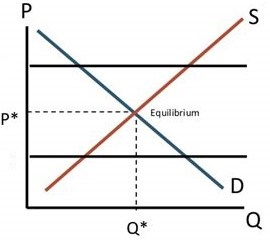
\includegraphics[width=6cm]{Images/Inkednon-labelled controls.jpg}
    \end{figure}
    \end{itemize}
\end{frame}

\begin{frame}{Effective Price Controls}
    \begin{itemize}[<+->]
    \item It's the opposite of what you might think: effective price floors are above equilibrium, effective price ceilings are below
    \begin{figure}
        \centering
        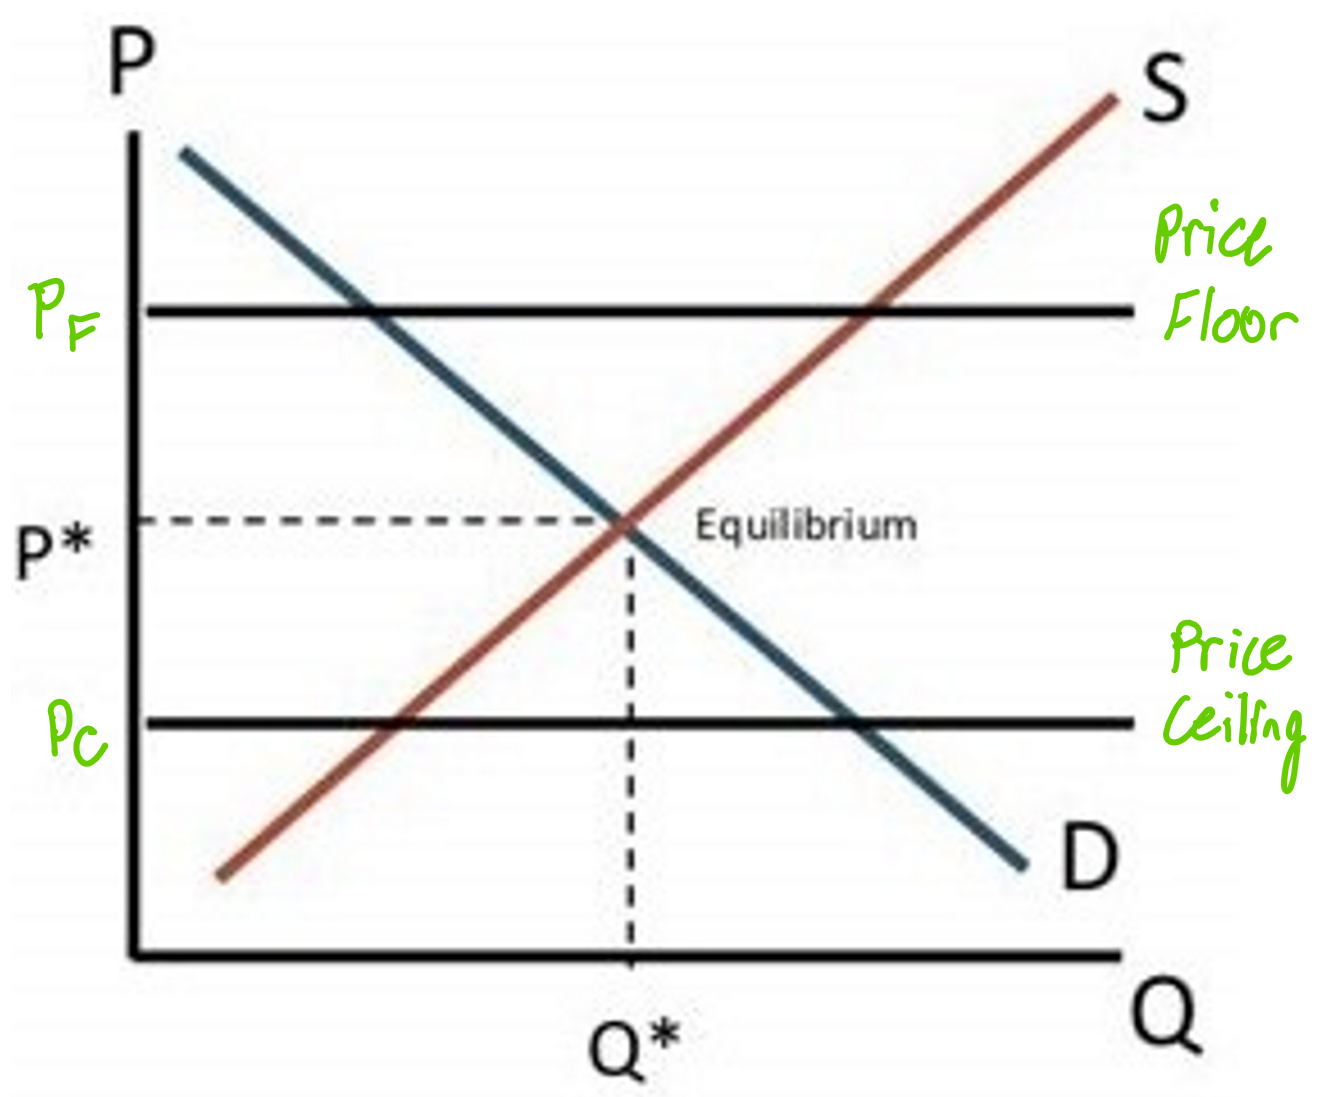
\includegraphics[width=6cm]{Images/labelled effective controls.png}
    \end{figure}
    \item Remember, that either of these could be a ceiling/floor, but if I tell you it's an ``\underline{effective}" ceiling floor, you can tell which is which
    \end{itemize}
\end{frame}

\section*{The Welfare Effects of Price Controls}

\begin{frame}{Example 1 -- Unregulated (Q)}
    \begin{itemize}[<+->]
    \item Consider the following market for MLB tickets
    \begin{figure}
        \centering
        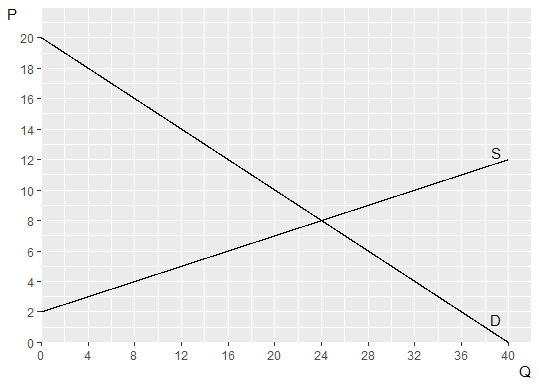
\includegraphics[width=8.5cm]{R MLB Plot.png}
        \vspace{-2mm}
    \end{figure}
    \item Compute CS, PS, and TS in this graph
    \end{itemize}
\end{frame}

\begin{frame}{Example 1 -- Unregulated (A)}
    \begin{itemize}[<+->]
    \item CS/PS are visualized as in the graph below:
    \begin{figure}
        \centering
        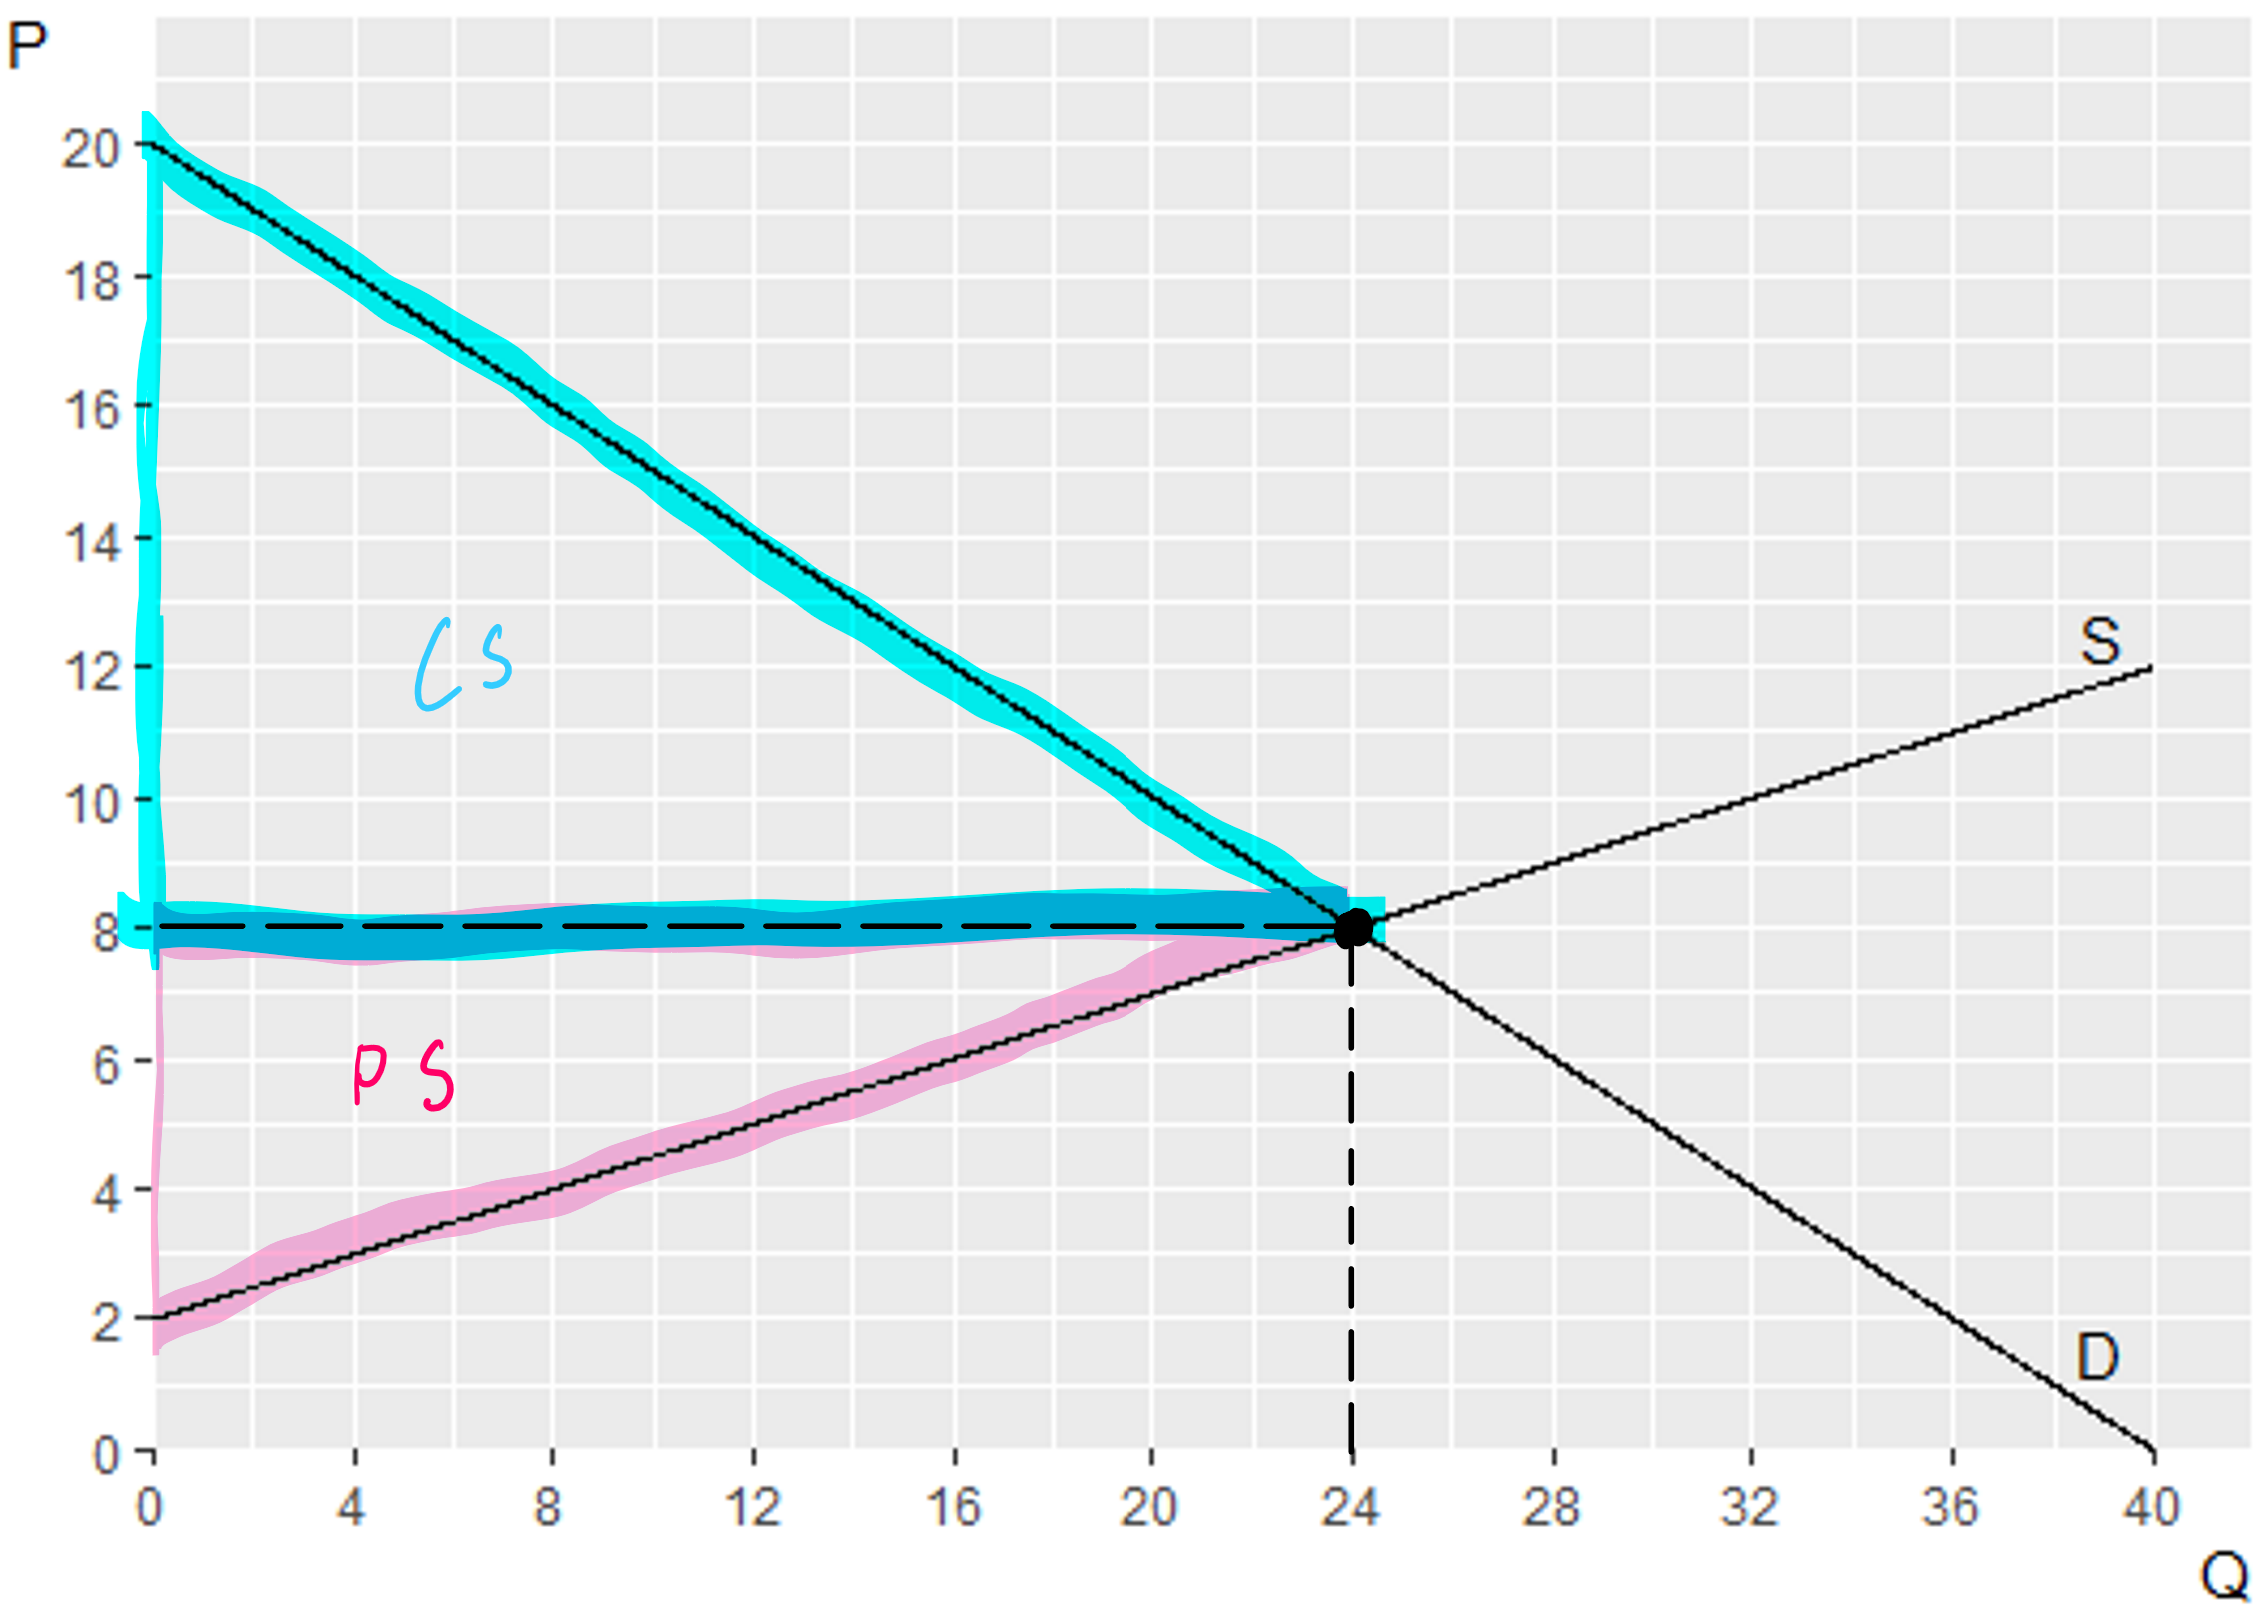
\includegraphics[width=6.5cm]{MLB unreg CS-PS.png}
    \end{figure}
    \item $CS=\frac{1}{2}(24)(20-8)=12(12)=144$
    \item $PS=\frac{1}{2}(24)(8-2)=12(6)=72$
    \begin{itemize}
        \item Therefore, $TS=216$
    \end{itemize}
    \end{itemize}
\end{frame}

\begin{frame}{Example 1 -- Price Floor}
    \begin{itemize}[<+->]
    \item Suppose, to protect producer interests, the league mandates a $\$12$ price floor on games
    \item Draw this price floor now\pause
    \begin{figure}
        \centering
        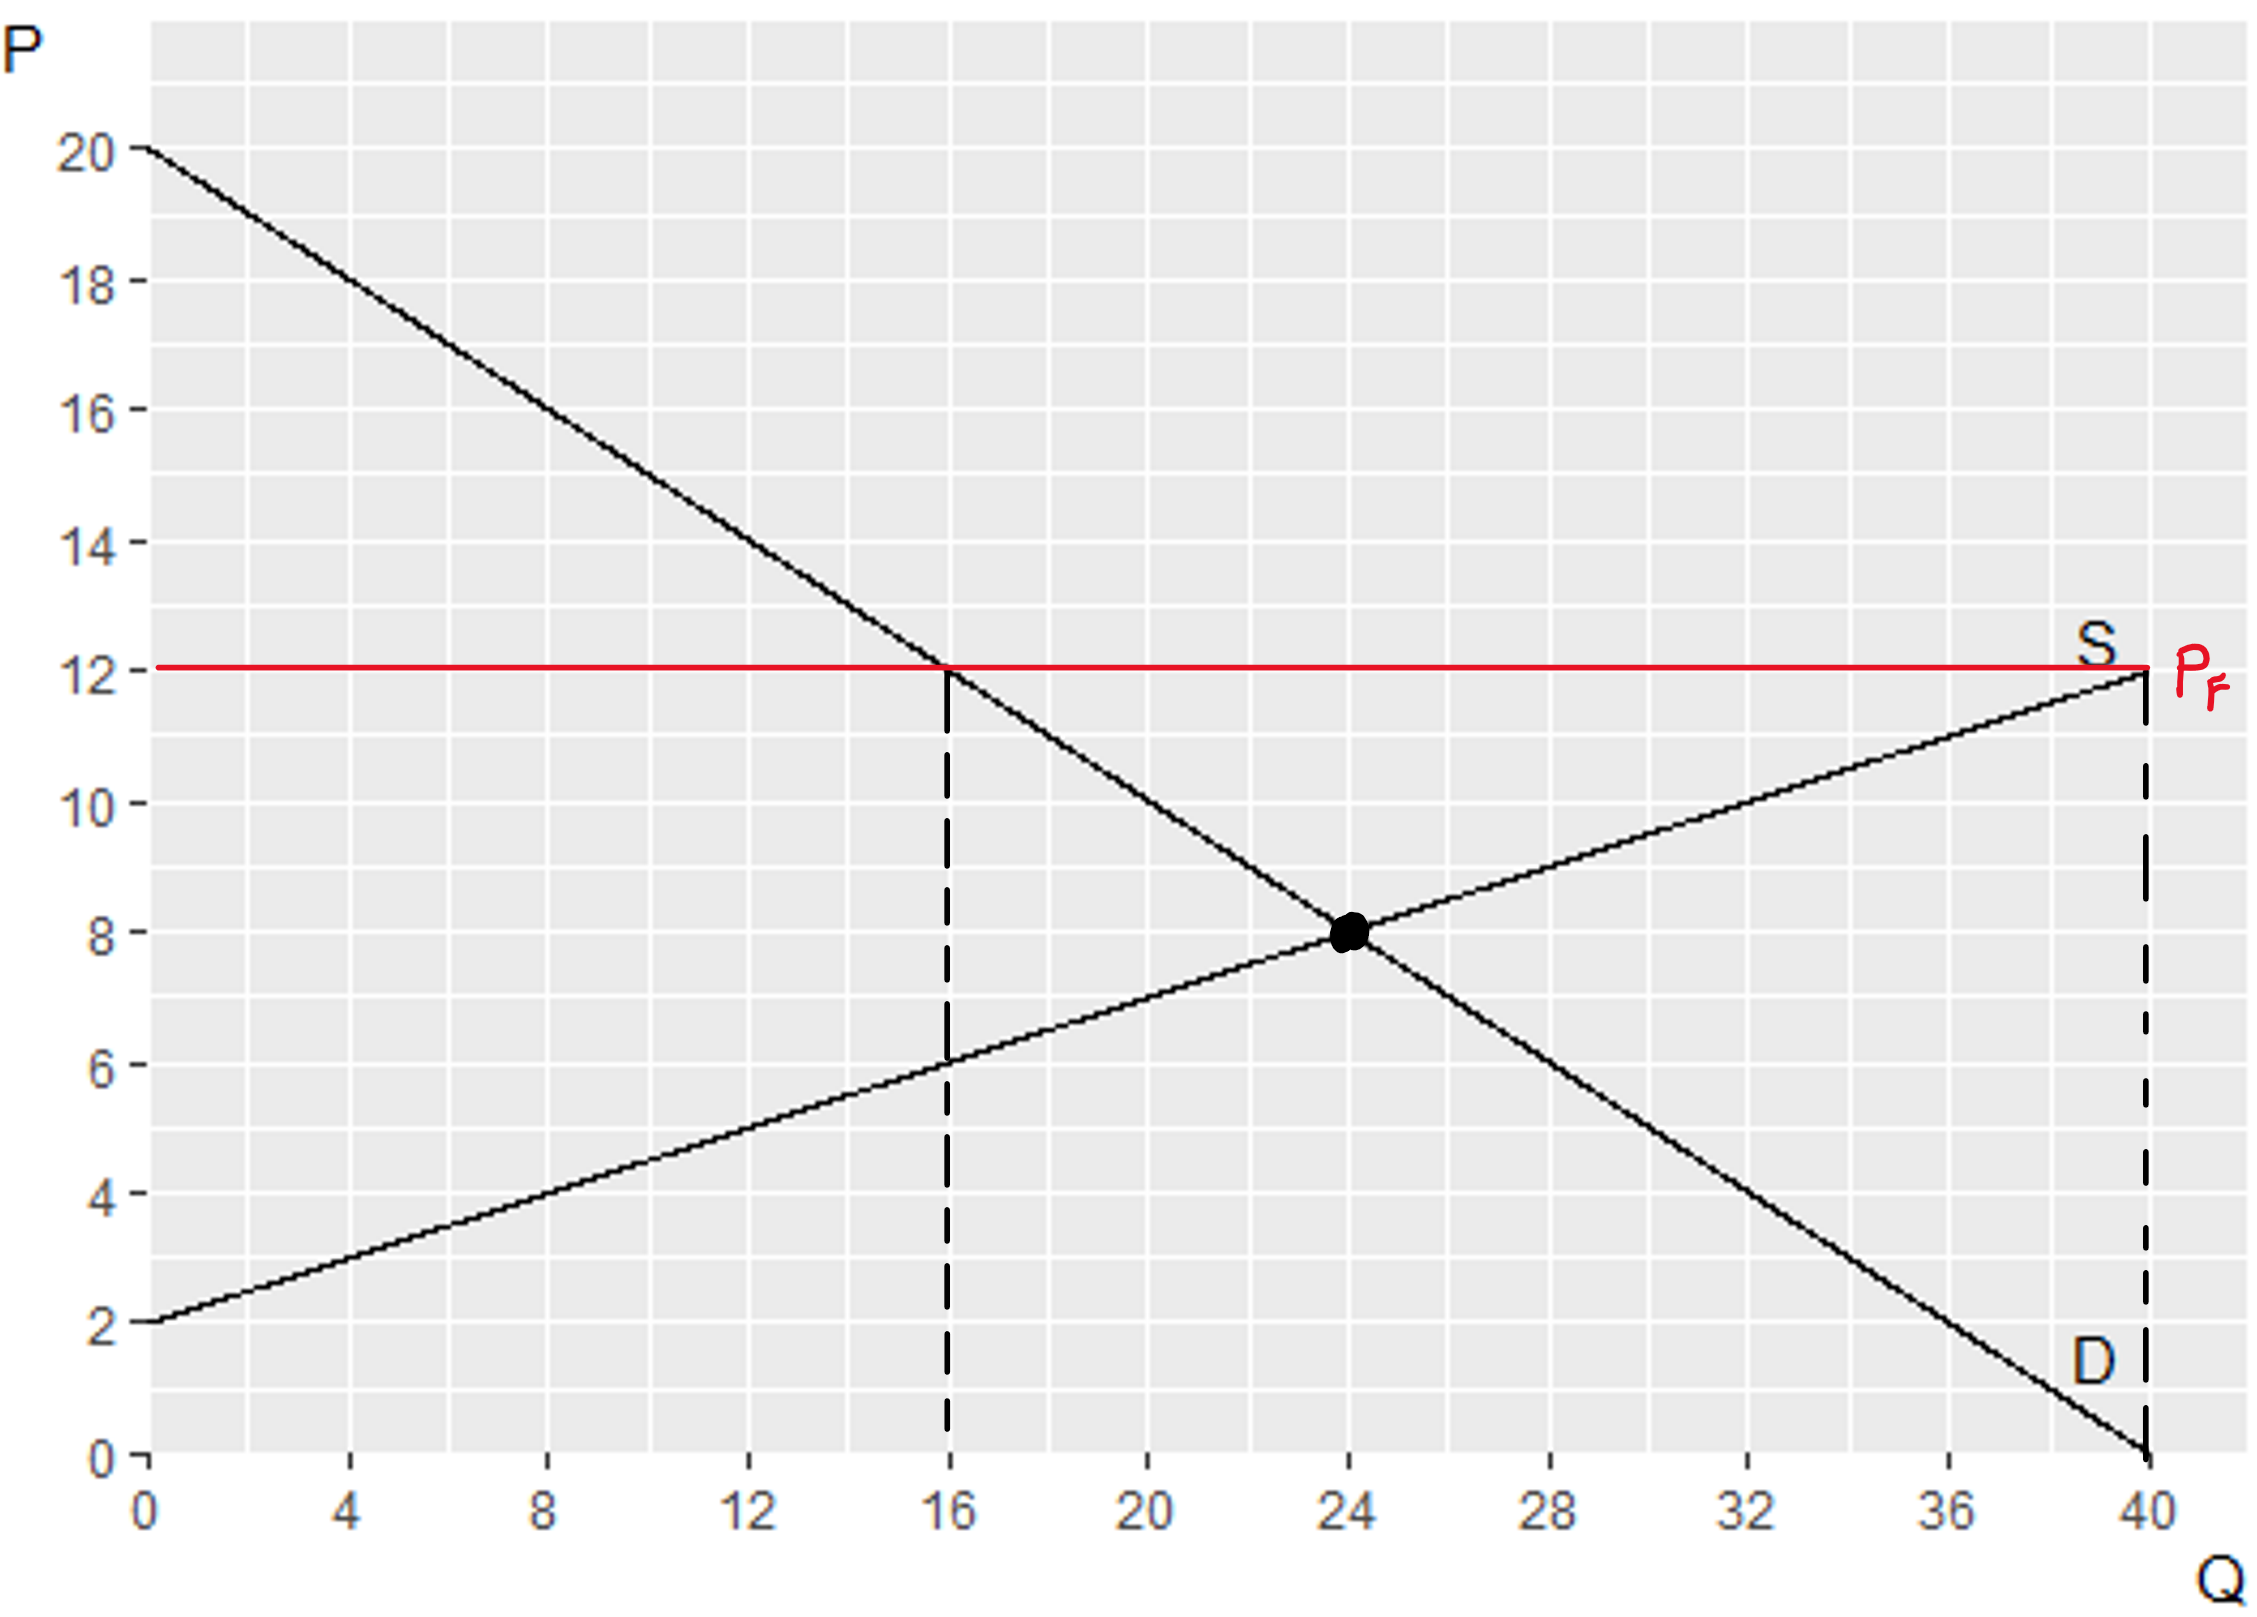
\includegraphics[width=5.5cm]{MLB price floor.png}
    \end{figure}
    \item Is this price floor effective?
    \begin{itemize}
        \item Yes, because it is above the equilibrium
    \end{itemize}
    \item What is quantity supplied? Quantity demanded?
    \begin{itemize}
        \item $Q_{D}=16$, $Q_{S}=40$
    \end{itemize}
    \end{itemize}
\end{frame}

\begin{frame}{Example 1 -- Price Floor (cont.)}
    \begin{itemize}[<+->]
    \item Suppose, to protect producer interests, the league mandates a $\$12$ price floor on games
    \item Draw this price floor now\pause
    \begin{figure}
        \centering
        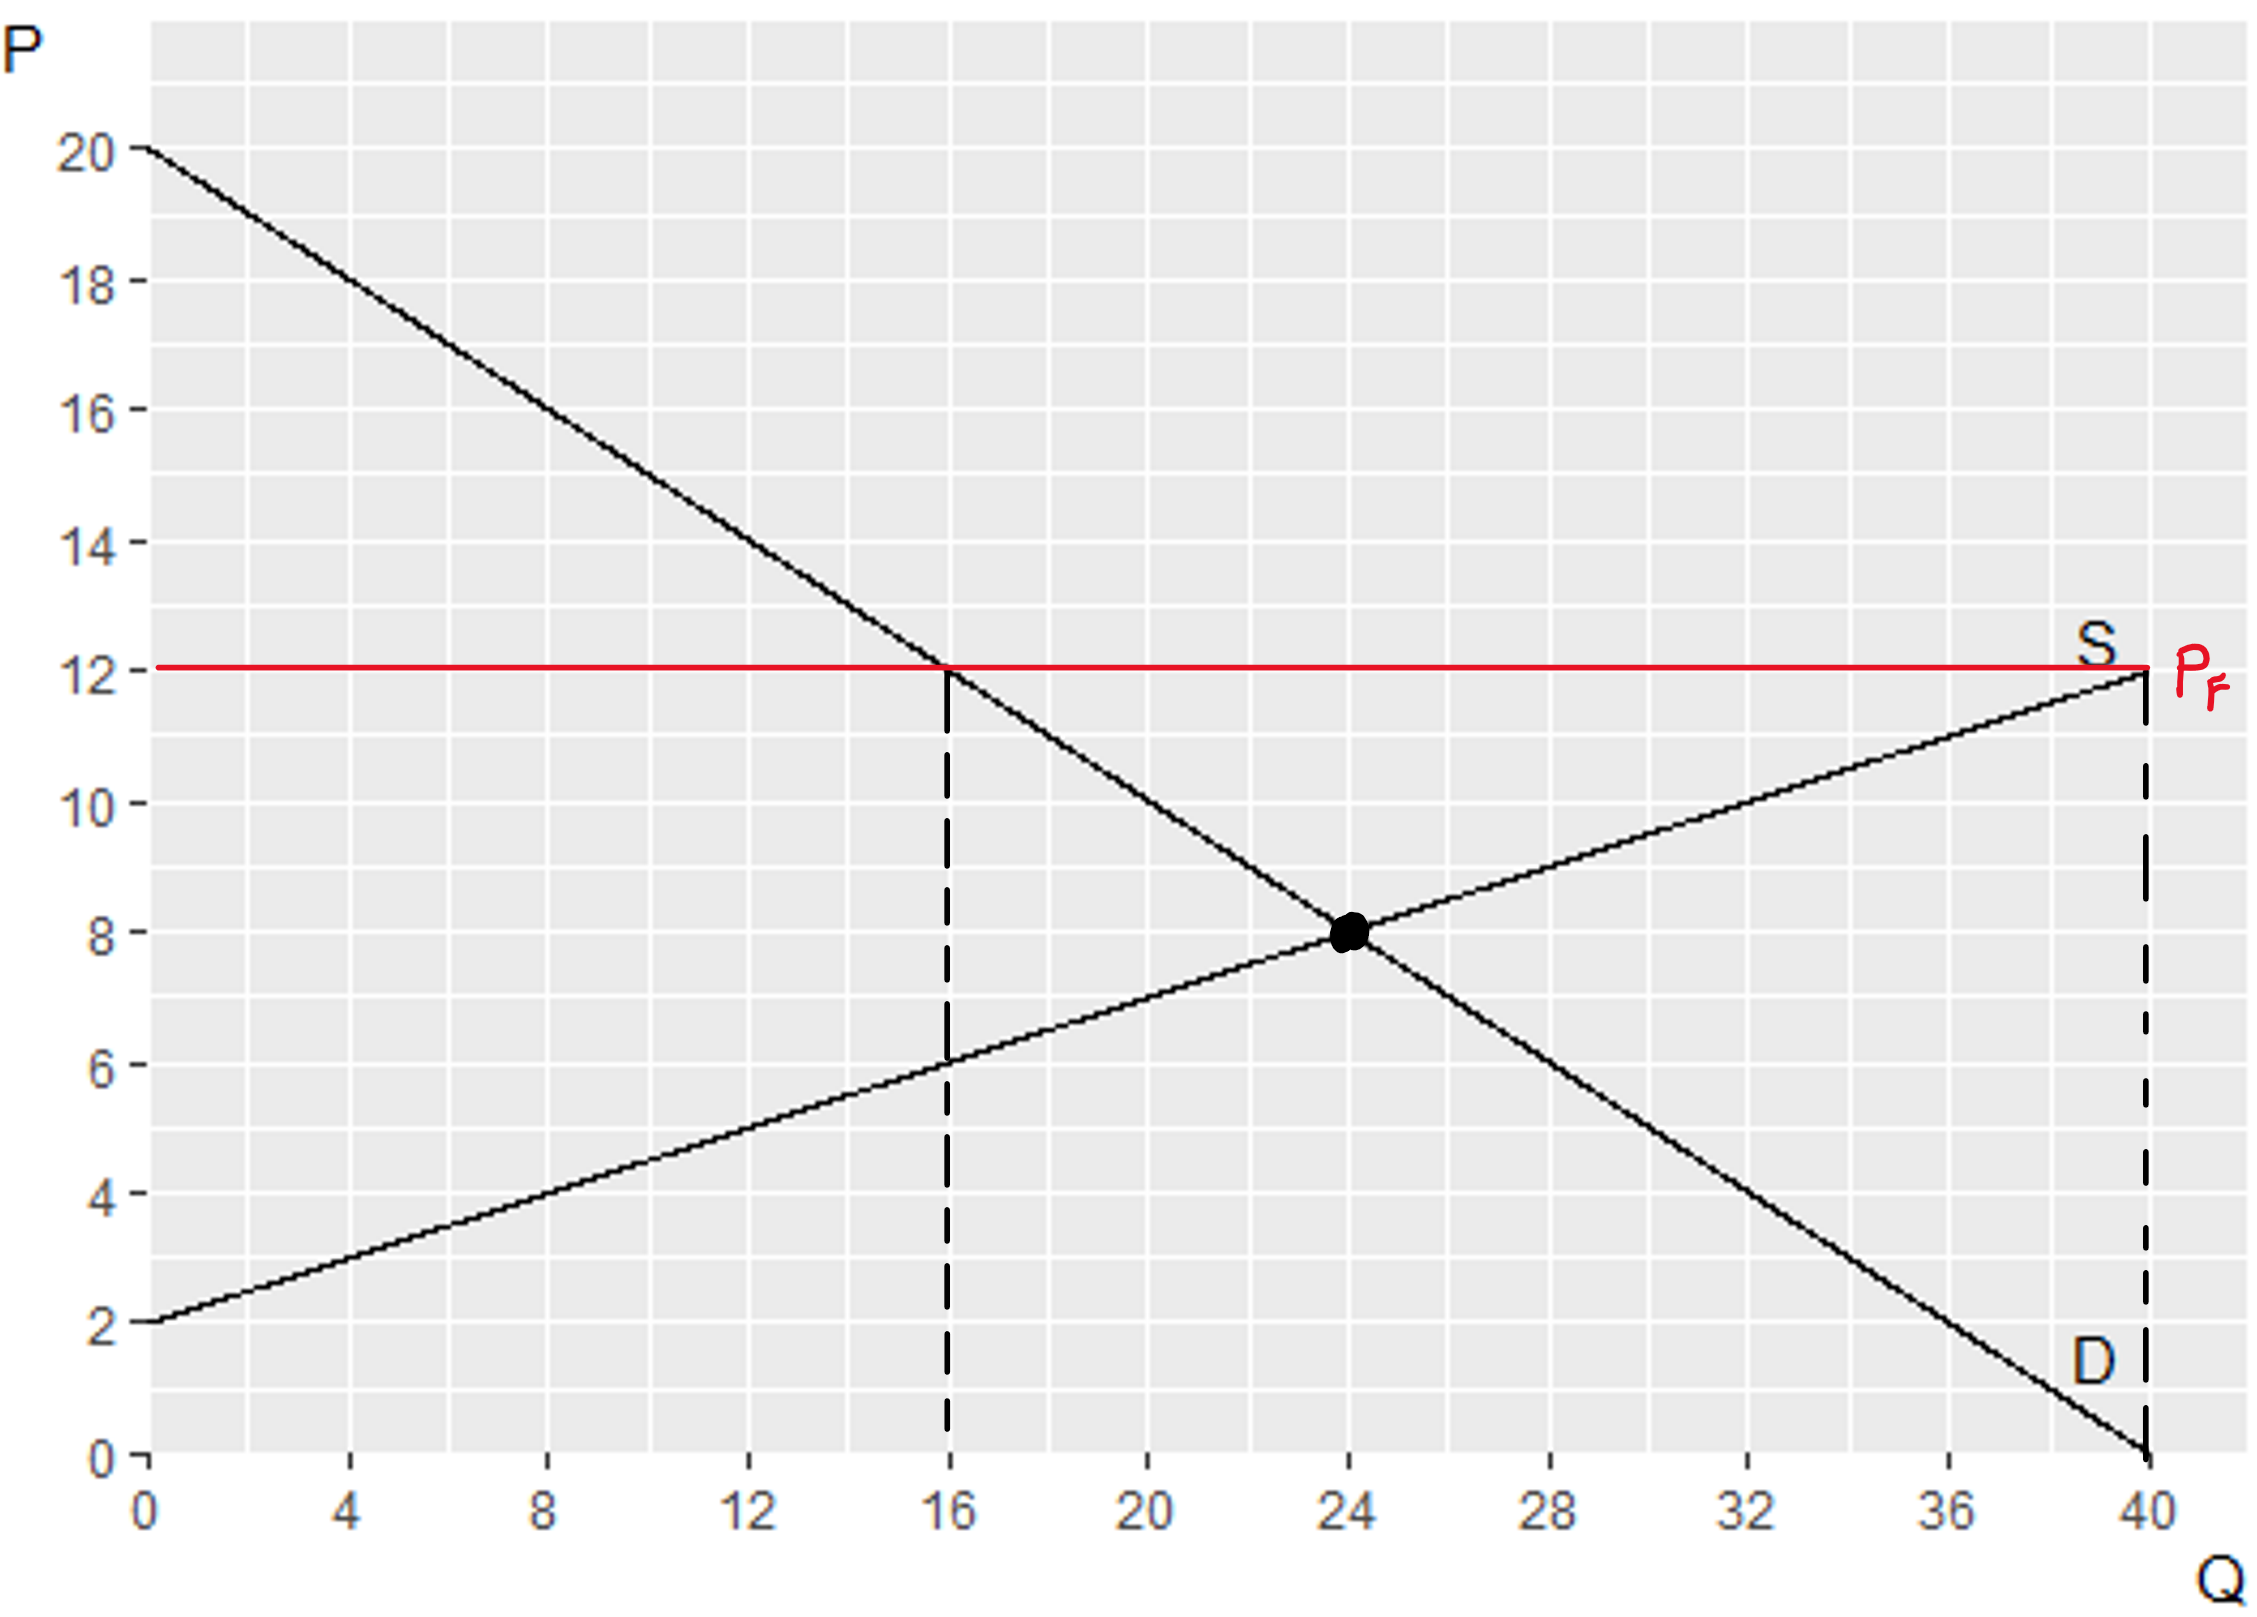
\includegraphics[width=5.5cm]{MLB price floor.png}
    \end{figure}
    \item How many tickets are being traded? 
    \begin{itemize}
        \item 16, because that is all that is being demanded at the new price ($\$12$)
    \end{itemize}
    \item Is there a shortage or a surplus? How big? 
    \begin{itemize}
        \item There is a surplus of $40-16=24$ tickets
    \end{itemize}
    \end{itemize}
\end{frame}


\begin{frame}{Example 1 -- New Surplus (Q)}
    \begin{itemize}[<+->]
    \item What are the new CS/PS on the graph?\pause
    \begin{figure}
        \centering
        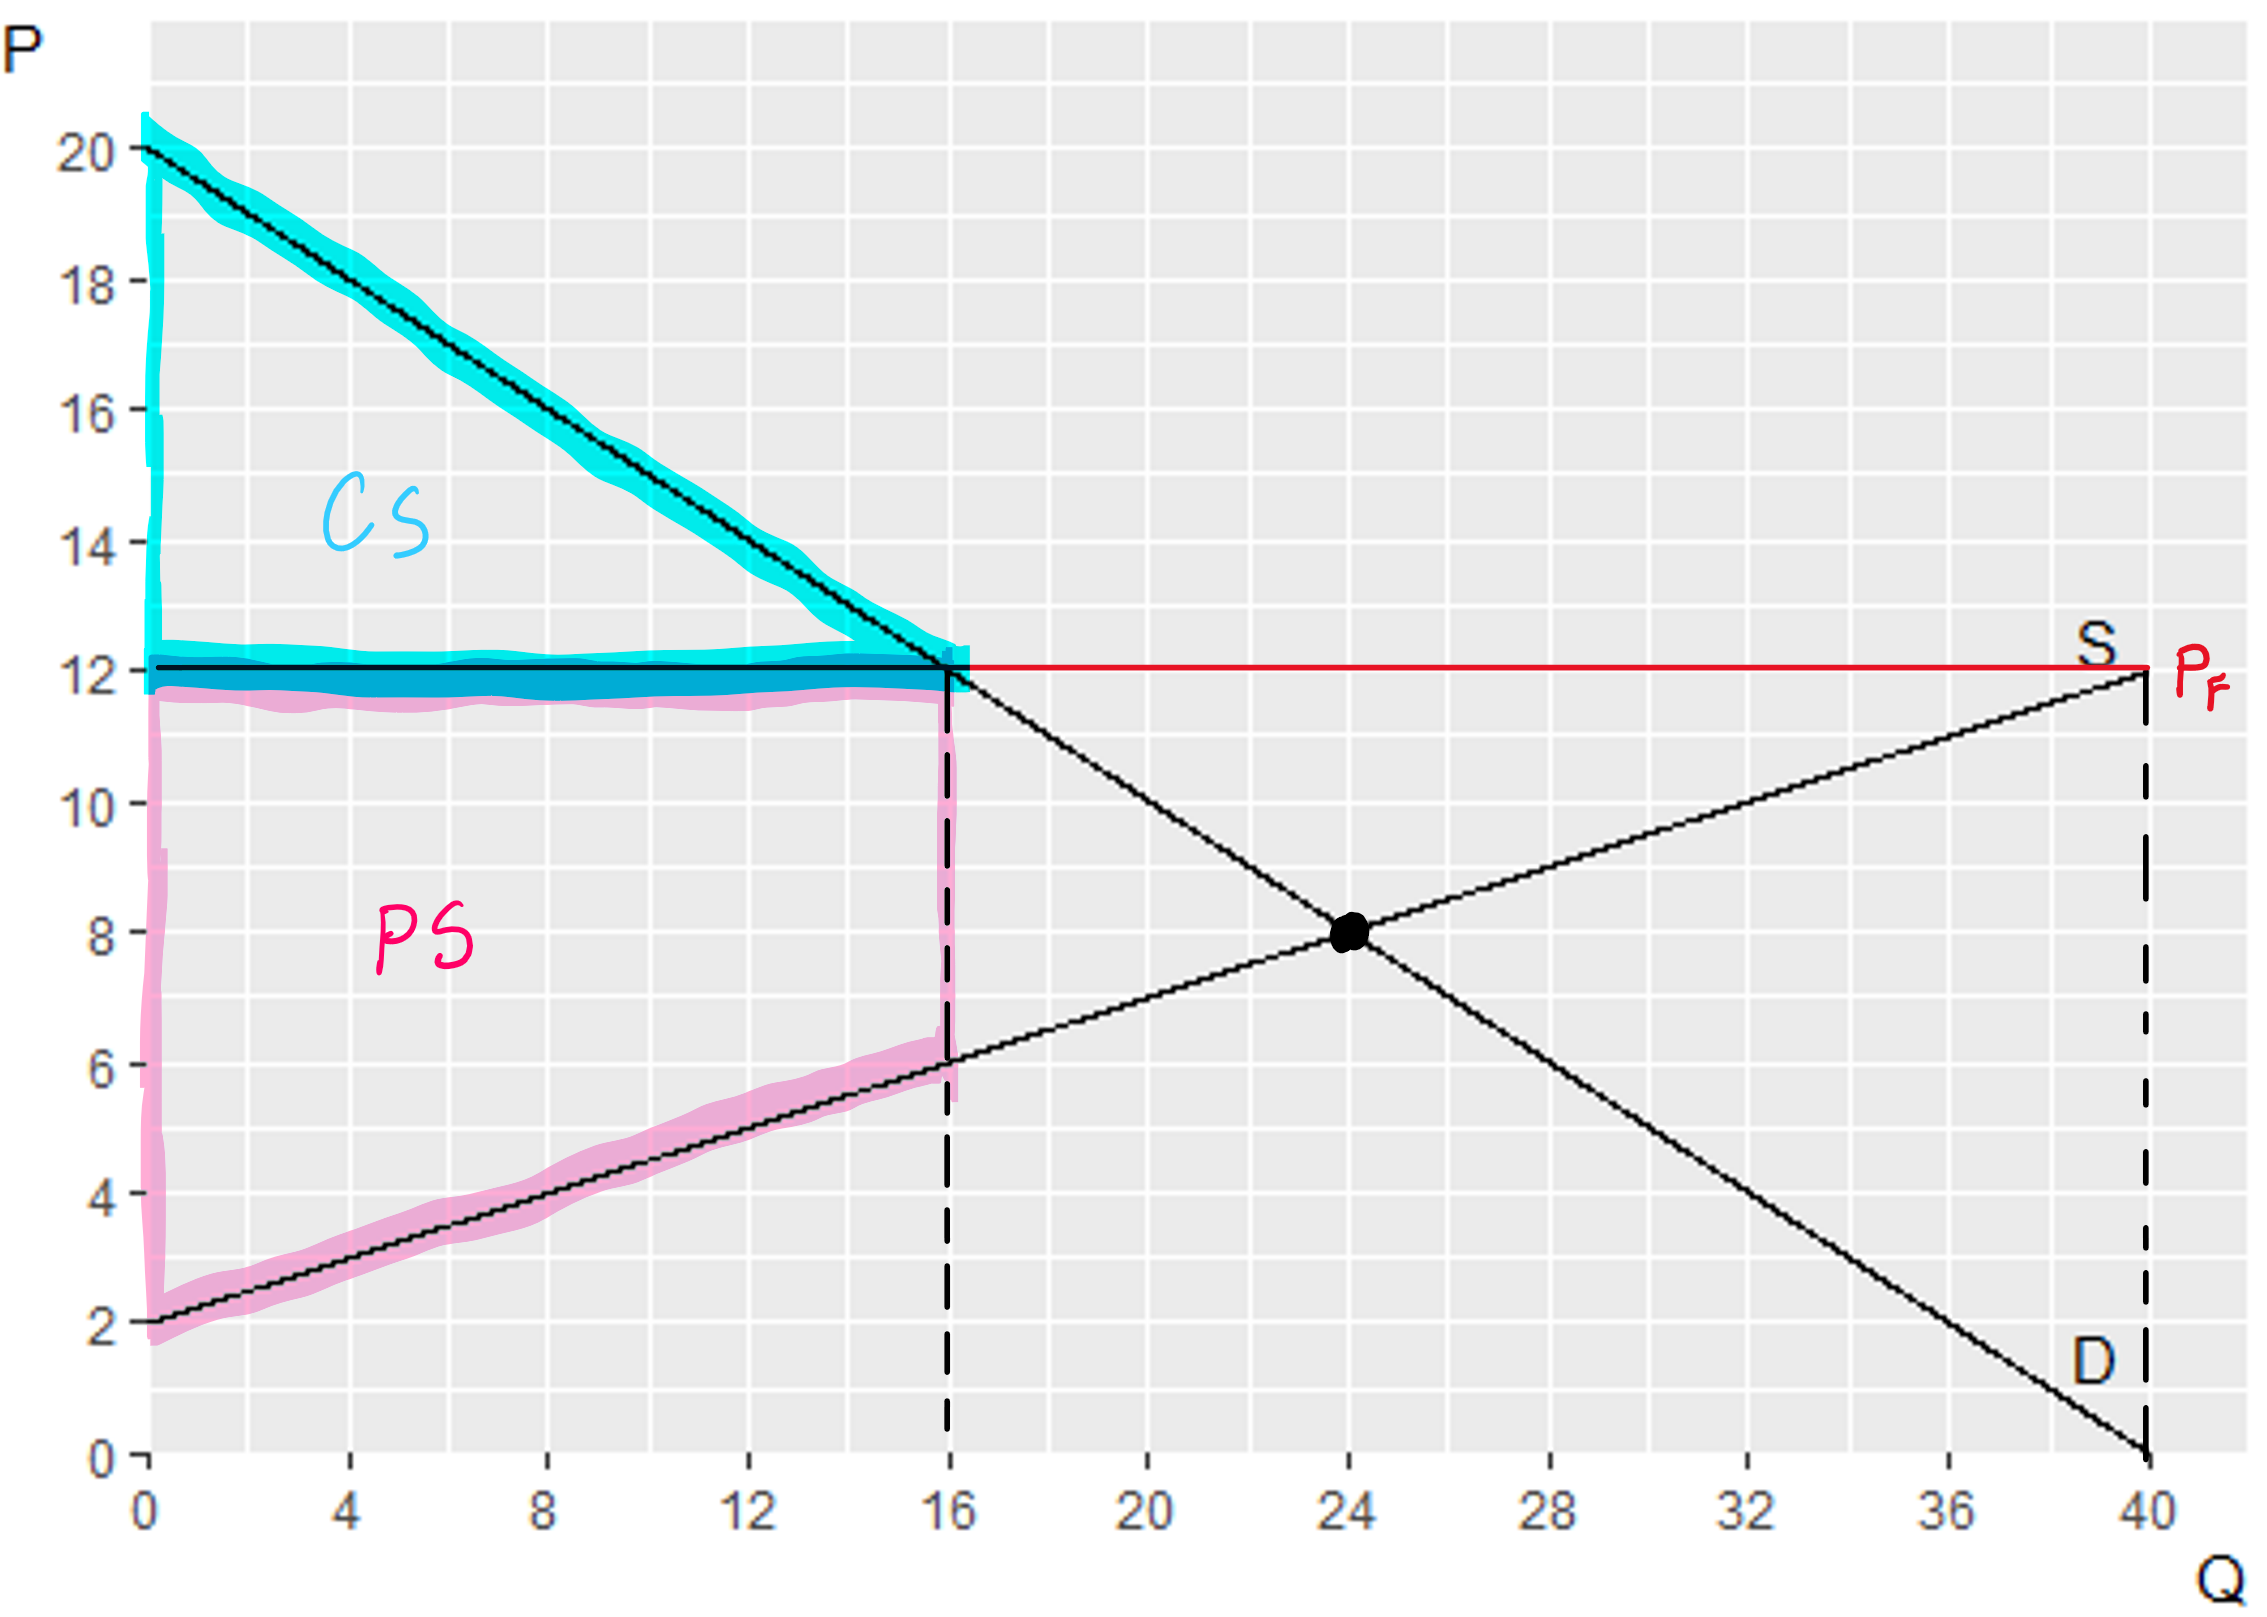
\includegraphics[width=5.5cm]{MLB reg CS-PS.png}
    \end{figure}
    \item Remember, the market is trading 16 tickets \@ $\$12$. So, from a quantity of 16, CS is the area between price ($\$12$) and demand, while PS is the area from supply to price
    \end{itemize}
\end{frame}

\begin{frame}{Example 1 -- New Surplus (A)}
    \begin{itemize}[<+->]
    \item What are the new CS/PS/TS?
    \begin{figure}
        \centering
        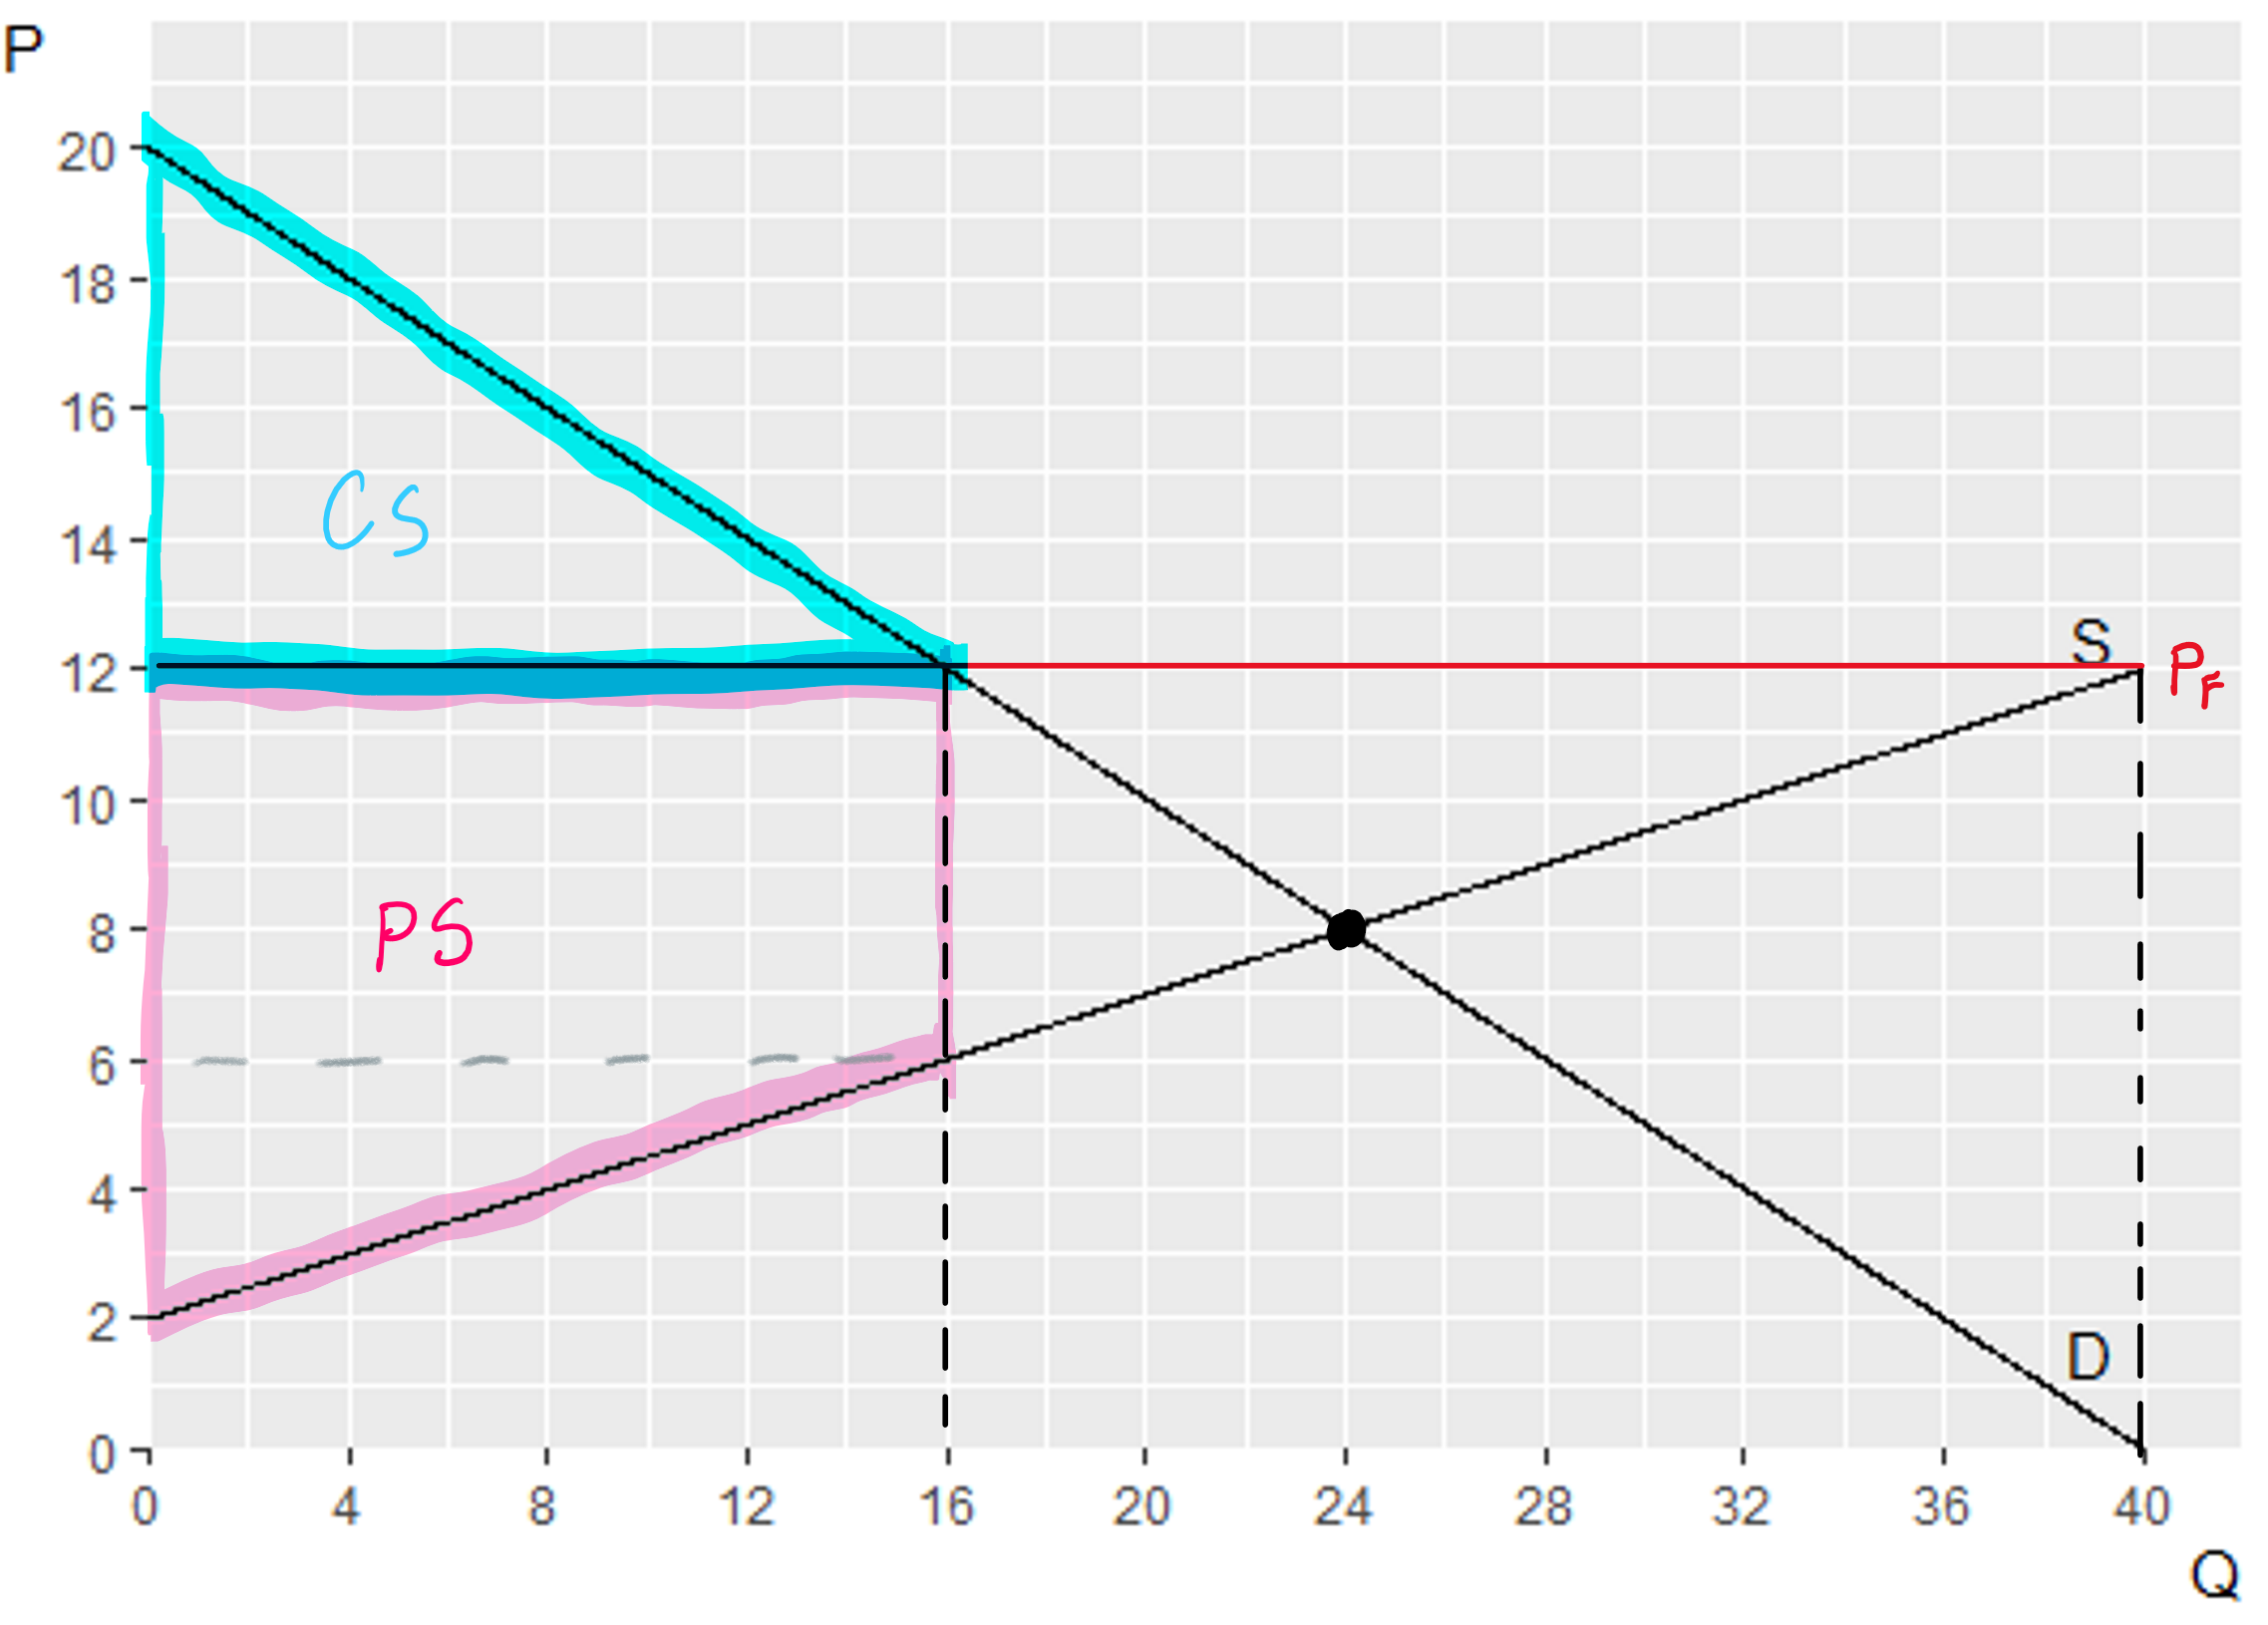
\includegraphics[width=5cm]{MLB reg CS-PS calculation.png}
    \end{figure}
    \item $CS=\frac{1}{2}(16)(20-12)=8(8)=64$
    \item $PS=\frac{1}{2}(16)(6-2) + (16)(12-6)=8(4)+16(6)=128$
    \begin{itemize}
        \item Therefore, TS is now 196
    \end{itemize}
    \end{itemize}
\end{frame}


\begin{frame}{Example 1 -- New Surplus (cont.)}
    \begin{itemize}[<+->]
    \item What is the change in CS/PS/TS?
    \begin{figure}
        \centering
        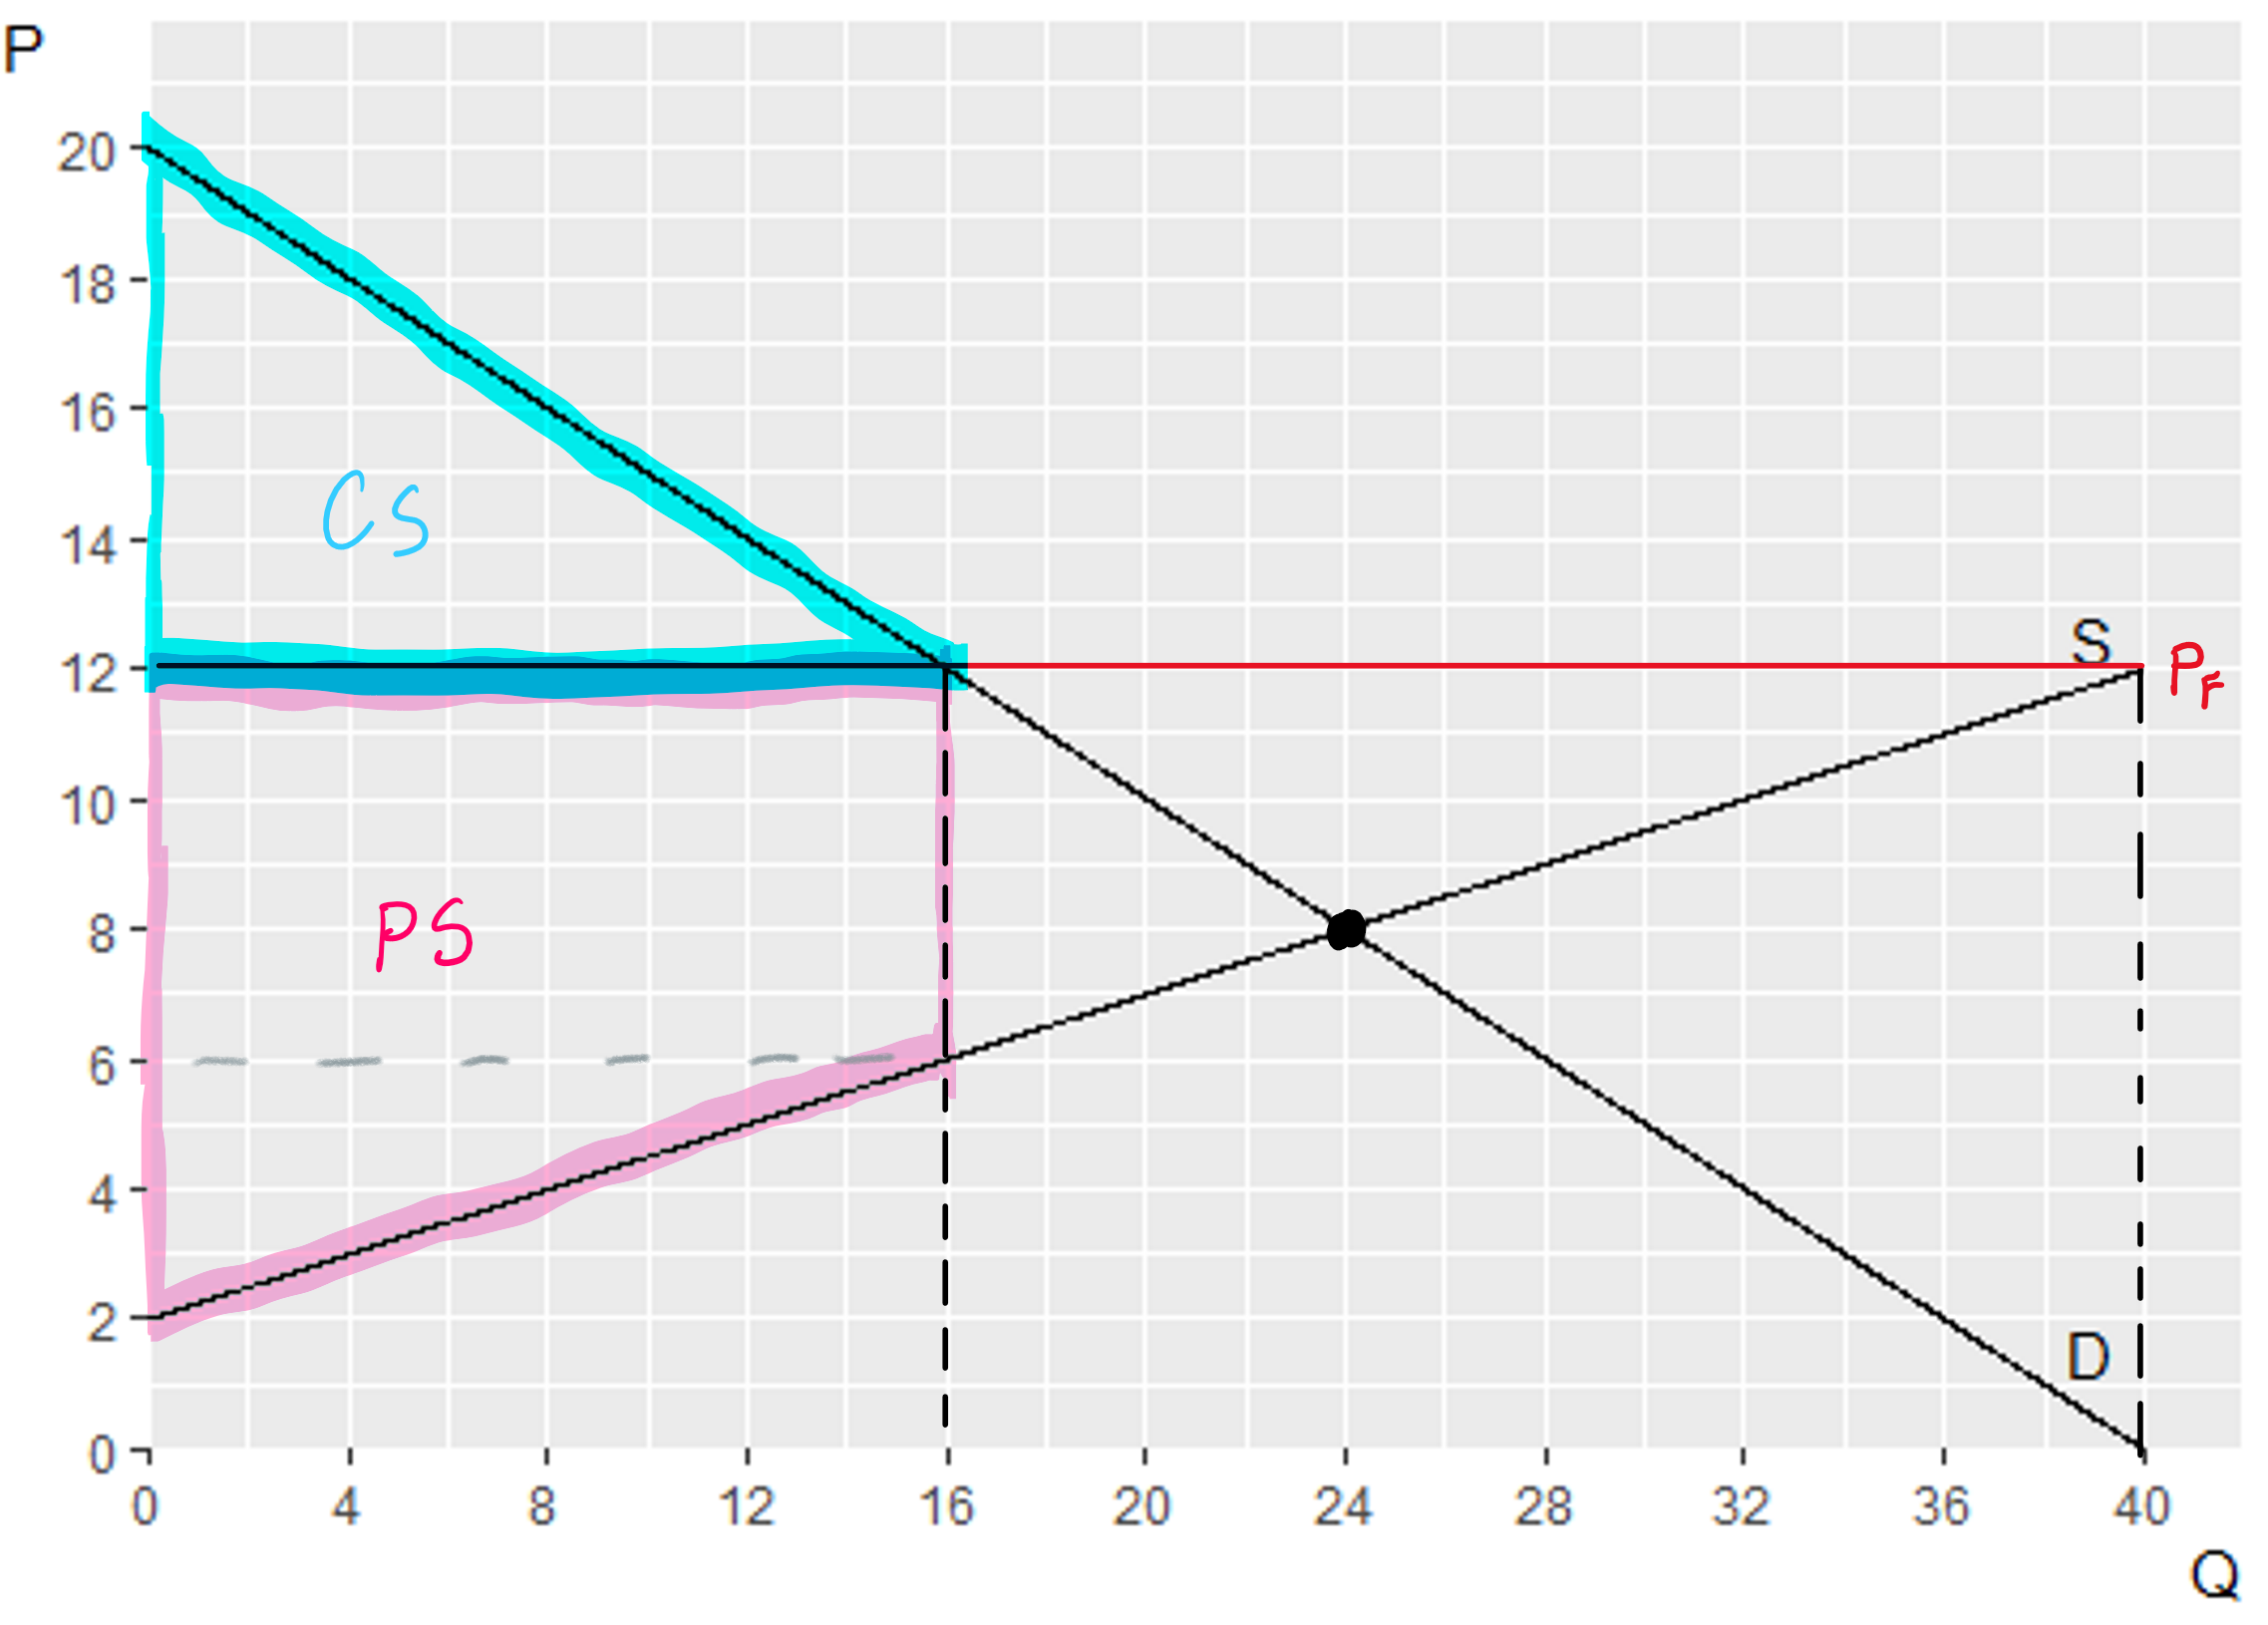
\includegraphics[width=4.5cm]{MLB reg CS-PS calculation.png}
    \end{figure}
    \item $\Delta CS=64-144=-80$
    \item $\Delta PS=128-72=56$
    \item $\Delta TS=176-216=-24$
    \vspace{2mm}
    \item That is: CS fell by 80 and PS grew by 56, so TS fell by a total of 24
    \end{itemize}
\end{frame}


\begin{frame}{Example 1 -- DWL}
    \begin{itemize}[<+->]
    \item What about the leftover area -- the difference between our unregulated TS and our regulated one?
    \begin{figure}
        \centering
        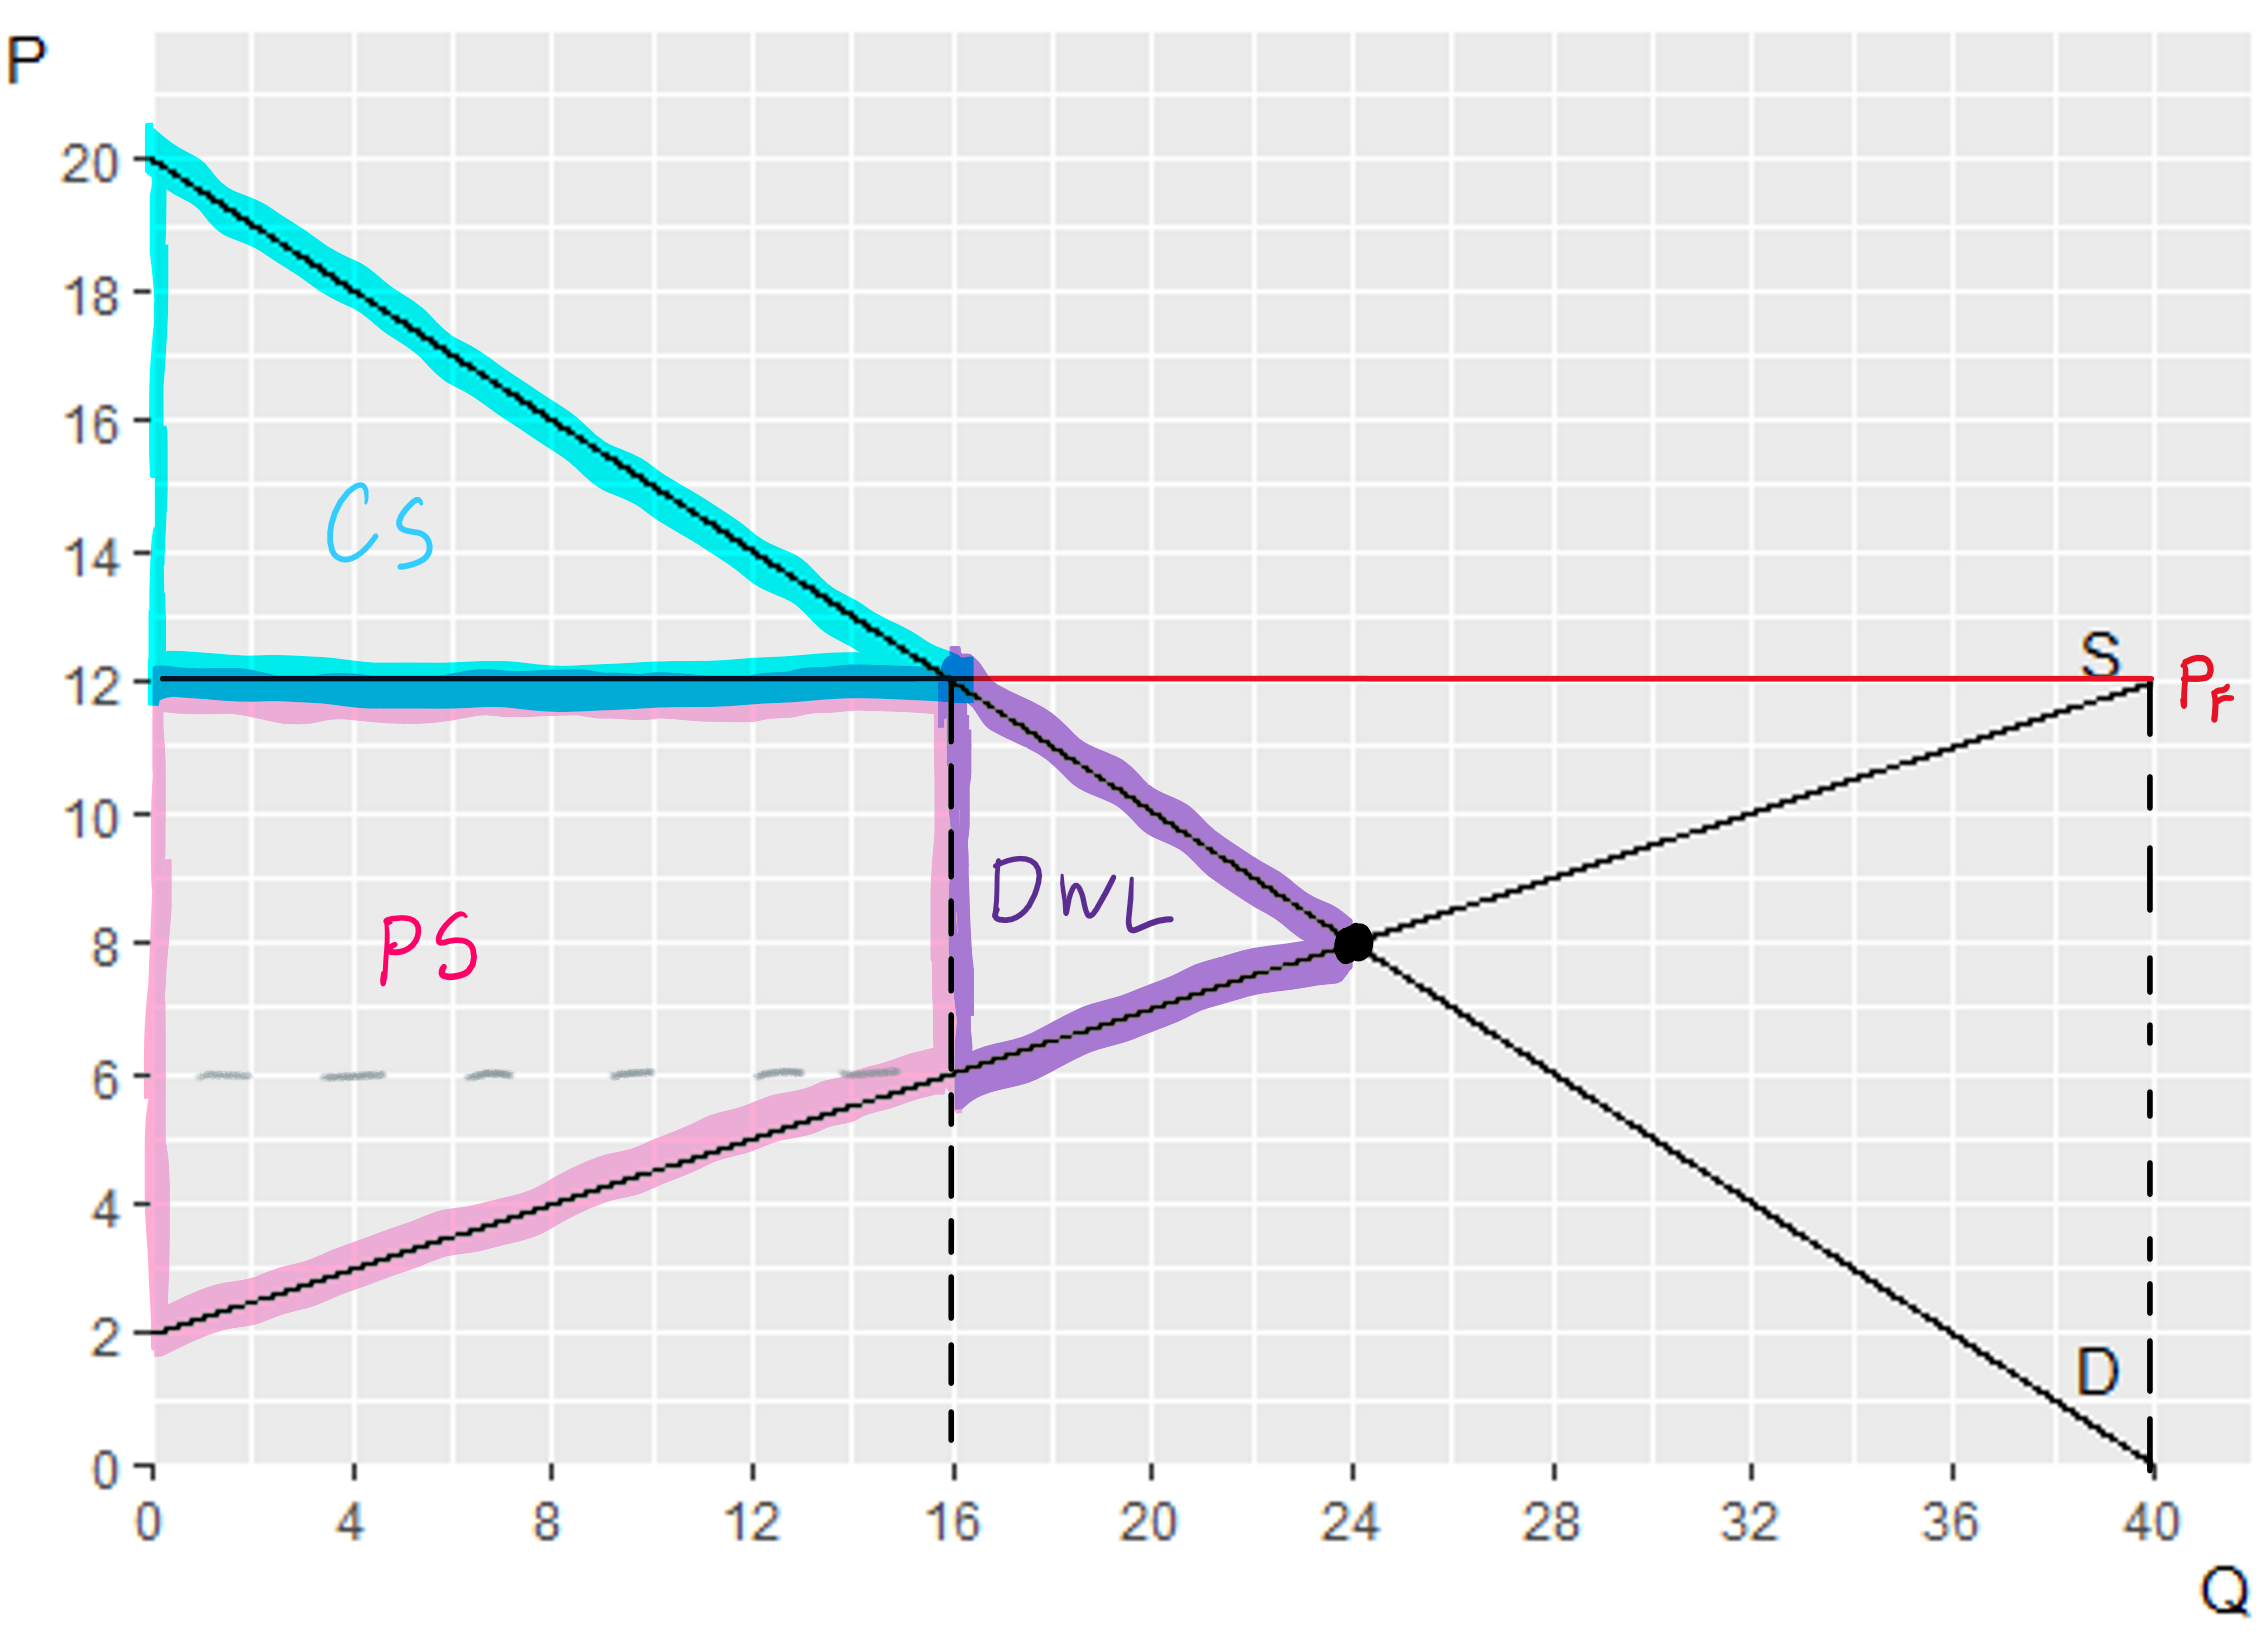
\includegraphics[width=6cm]{MLB DWL.png}
    \end{figure}
    \item This is called the \underline{Dead Weight Loss} (DWL), and will be frequent in the diagrams we explore over the next few classes
    \end{itemize}
\end{frame}

\begin{frame}{Deadweight Loss Definition}
    \begin{itemize}[<+->]
    \item The book defines \underline{{Deadweight Loss}} (DWL) as ``the fall in total surplus that results from a market distortion"
    \item I think a more accurate definition of  \underline{\textbf{Deadweight Loss}} (DWL) is the difference in total surplus between an efficient market and an inefficient one
    \begin{itemize}
        \item I make this subtle distinction, because when we get to externalities, taxes and subsidies can actually \textit{help} a market reach efficiency, but we aren't there yet
    \end{itemize}
    \item In nearly all of our figures in which deadweight loss occurs, it will be represented by a triangle
    \end{itemize}
\end{frame}

\begin{frame}{Example 1 -- DWL}
    \begin{itemize}[<+->]
    \item What is the are of DWL in our example?
    \begin{figure}
        \centering
        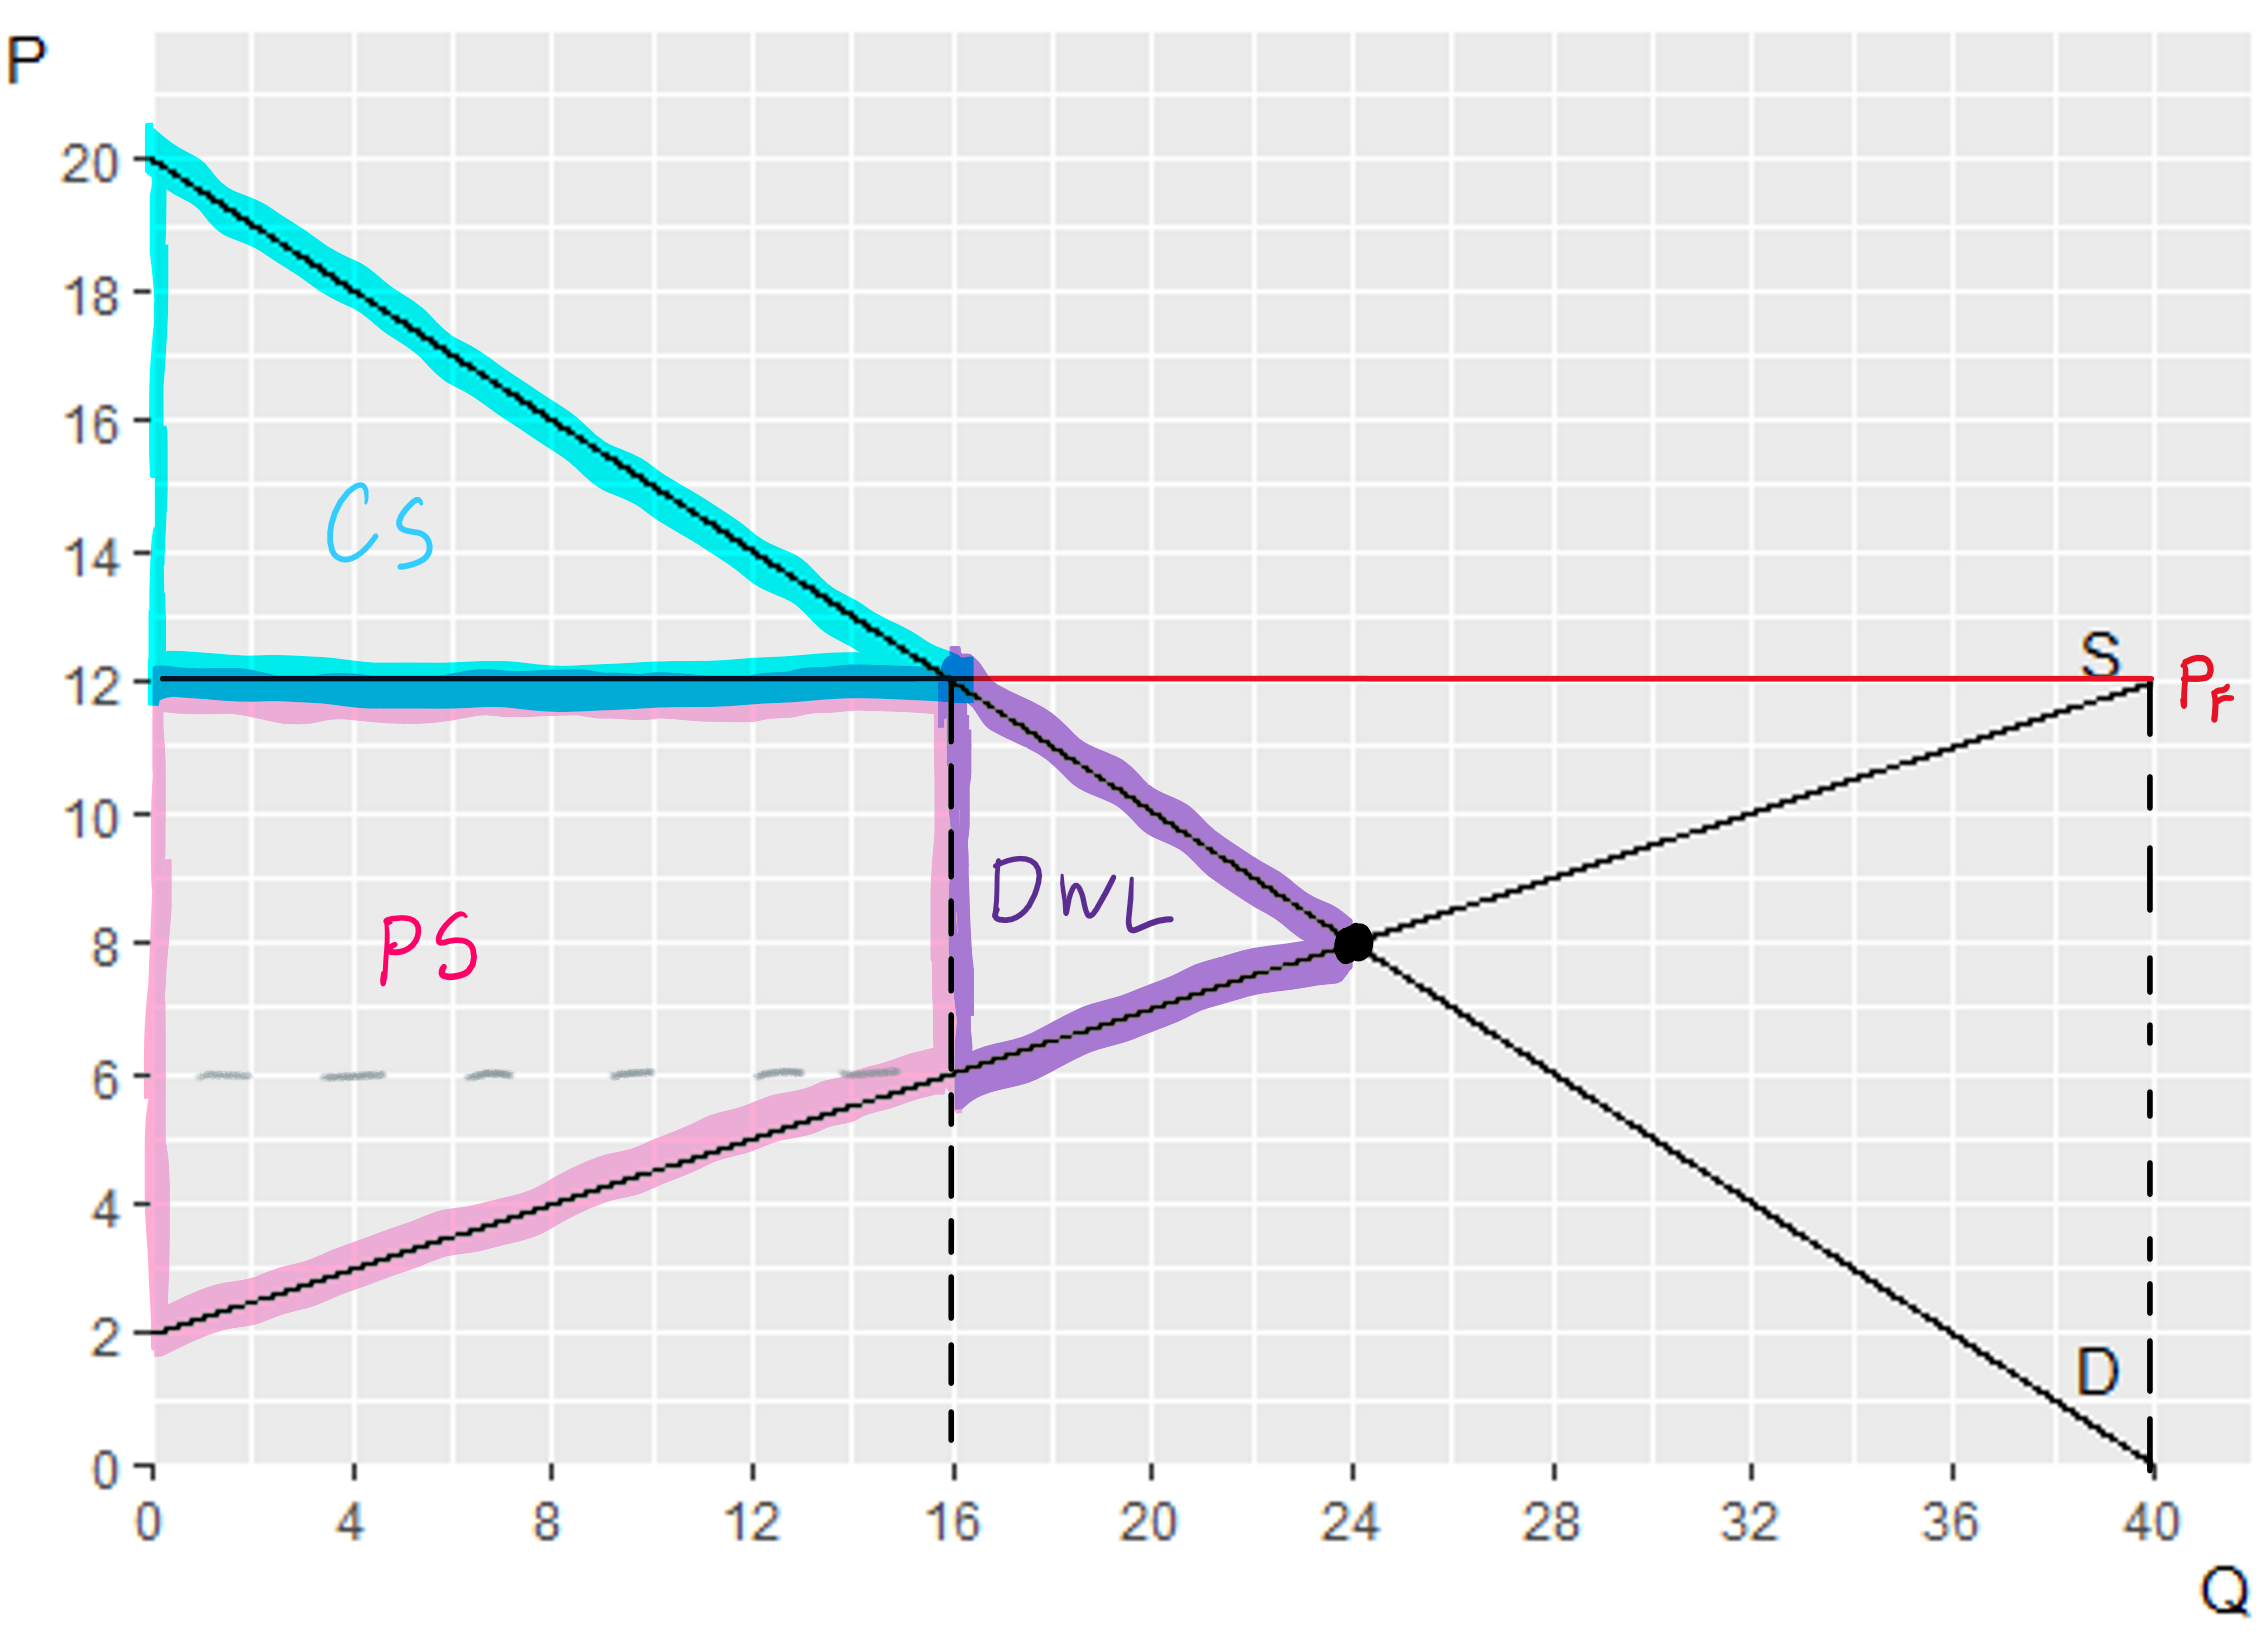
\includegraphics[width=6cm]{MLB DWL.png}
    \end{figure}
    \item $DWL=\frac{1}{2}(24-16)(12-6)=4(6)=24$
    \end{itemize}
\end{frame}



\section*{Elasticity and Surplus}

%Give the students enough to look at a new problem and characterize surplus and/or price effects
\begin{frame}{Example 1: Mutually Elastic Supply}
    \begin{itemize}[<+->]
        \item Consider a market in which consumers and producers are both relatively elastic (what does this mean?)
        \begin{itemize}
            \item Recall that this means that both consumers and producers are sensitive to prices
            \item The picture you should have in your head is grumbly consumers and producers who will rapidly exit the market if the price changes by a little bit 
        \end{itemize}
        \item To be explicit, 
        \begin{align*}
            [D]: \quad P&=189-\frac{1}{10}Q\\
            [S]: \quad P&=171+\frac{1}{10}Q
        \end{align*}
        \item What does this look like?
    \end{itemize}
\end{frame}


\begin{frame}{Example 1: Mutually Elastic Supply (Graph)}
        \begin{figure}
            \centering
            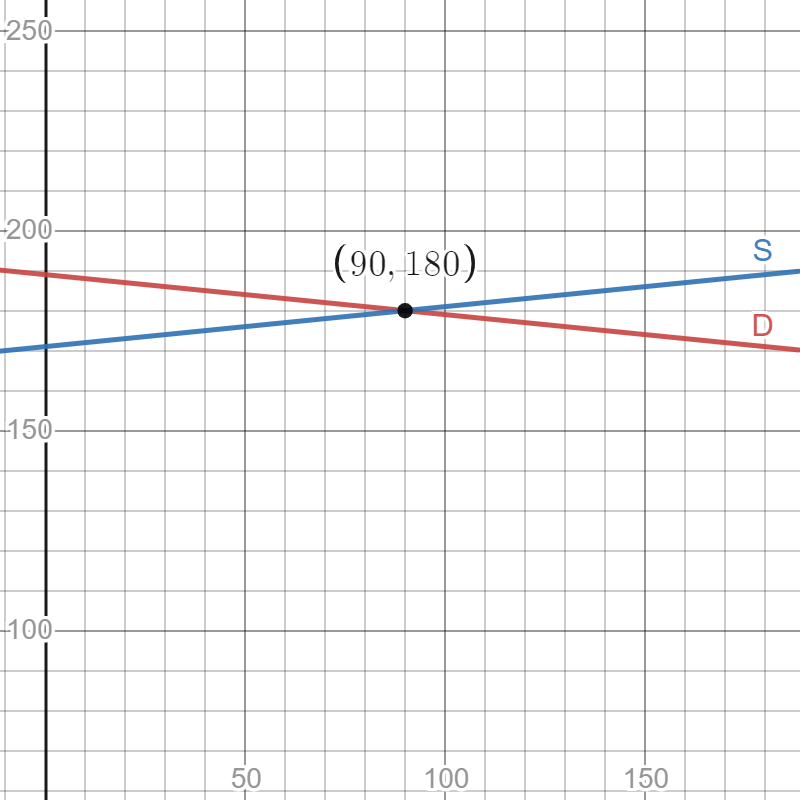
\includegraphics[width=5cm]{desmos mutual elastic.png}
        \end{figure}
    \begin{itemize}[<+->]
        \item What do CS and PS look like in the picture above?
        \item Relatively small
    \end{itemize}
\end{frame}


\begin{frame}{Example 1: Mutually Elastic Supply (Computation)}
\begin{table}
\centering
\renewcommand{\arraystretch}{3}
\begin{tabu}{cc}
    \multirow{2}[2]{*}[2mm]{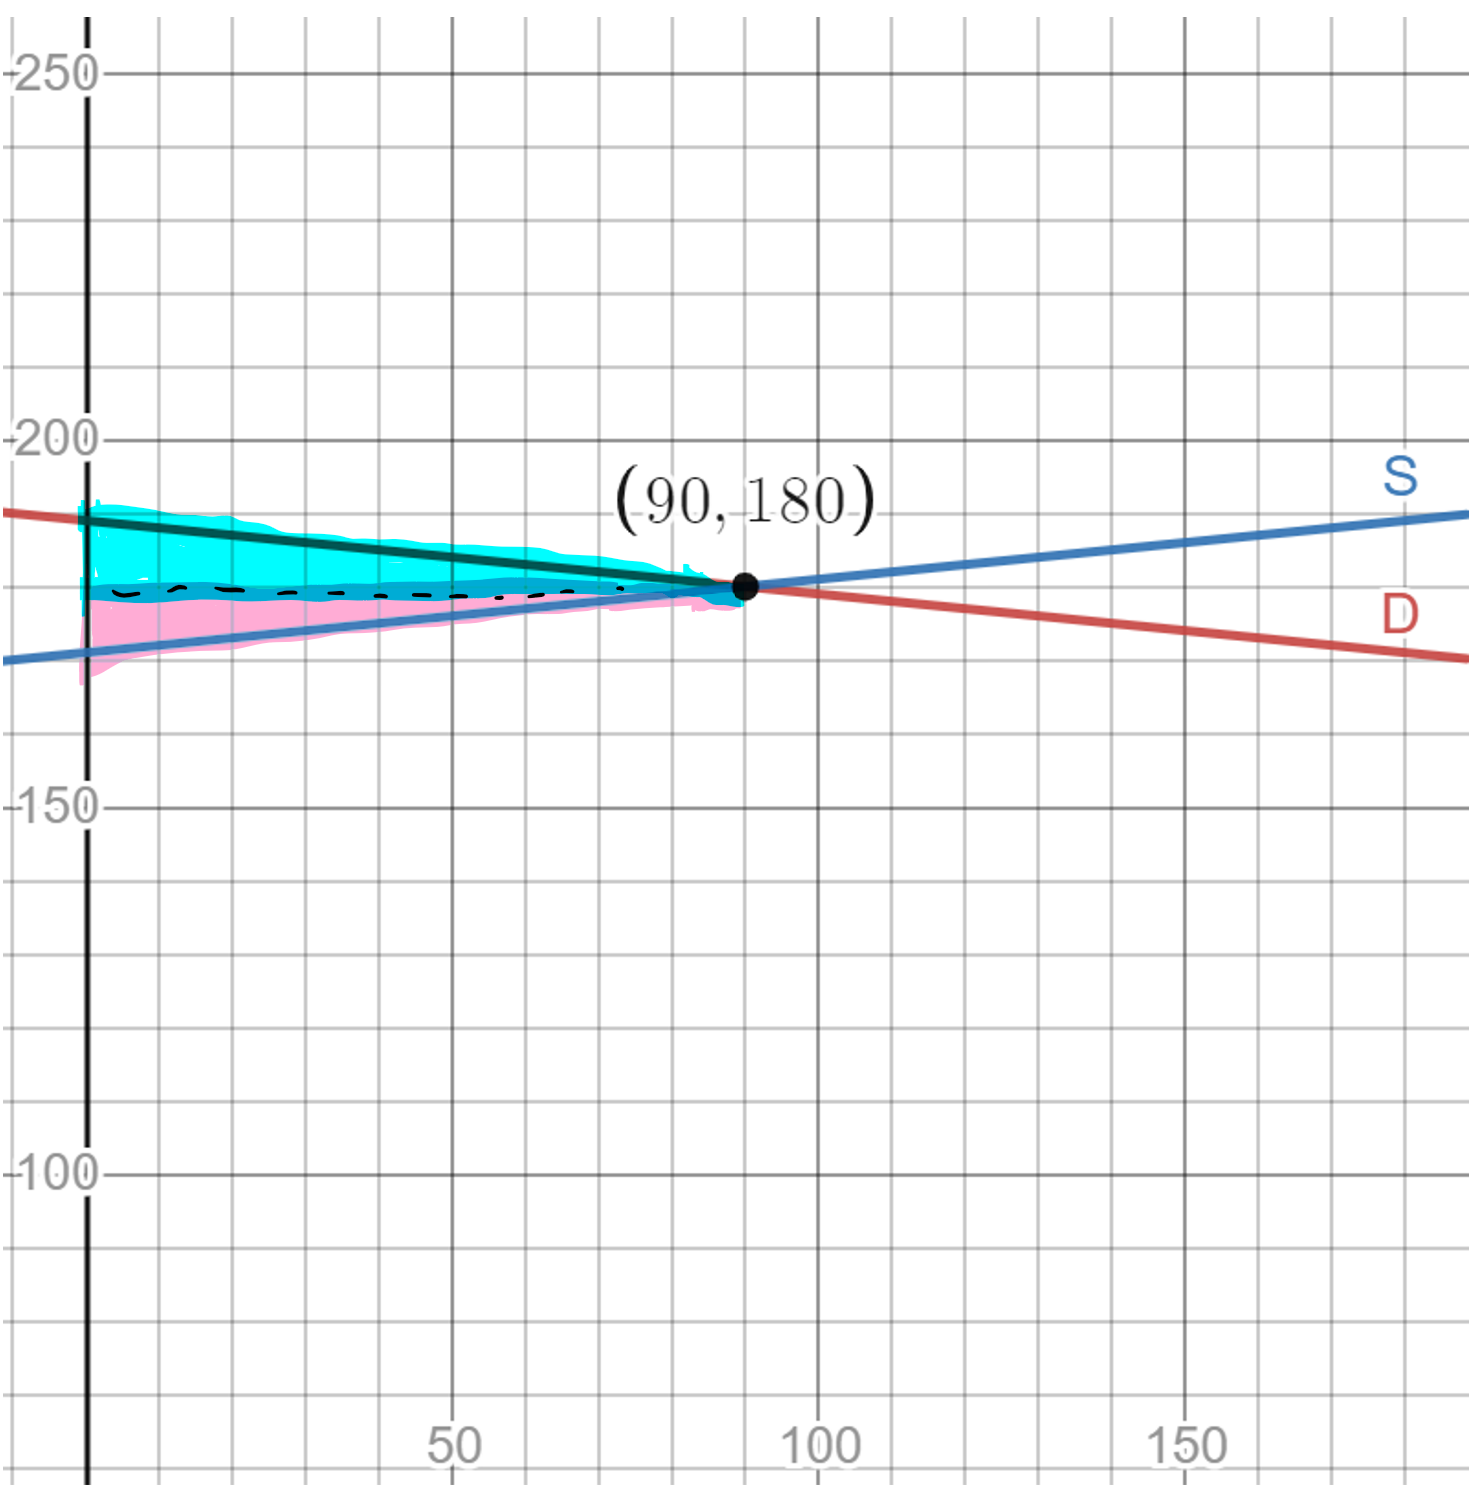
\includegraphics[width=4cm]{desmos mutual elastic CS-PS.png}} & $[D]: \quad P=189-\frac{1}{10}Q$ \bigstrut \\
    & $[S]: \quad P=171+\frac{1}{10}Q$ \bigstrut\\
\end{tabu}
\end{table}
\vspace{8mm}
    \begin{itemize}[<+->]
        \item $CS=\frac{1}{2}(90)(189-180)=405$
        \item $PS=\frac{1}{2}(90)(180-171)=405$
        \item What's happening: both consumers and producers are very sensitive to the price of the good: since small deviations cause lots of people to leave, both must agree on a price that does not suit the other greatly
    \end{itemize}
\end{frame}
    
    
\begin{frame}{Example 2: Mutually Inelastic Supply}
    \begin{itemize}[<+->]
        \item Now consider a market in which consumers and producers are both relatively inelastic
        \begin{itemize}
            \item Thus, consumers and producers are relatively \underline{insensitive} to prices
            \item The picture you should have in your head is consumers who really like and value the product, with a high WTP and and willingness to adapt to the price, and producers who can cheaply make a good, and really like doing it
        \end{itemize}
        \item To be explicit, 
        \begin{align*}
            [D]: \quad P&=360-2Q\\
            [S]: \quad P&=2Q
        \end{align*}
    \end{itemize}
\end{frame}


\begin{frame}{Example 2: Mutually Inelastic Supply (Graph)}
        \begin{figure}
            \centering
            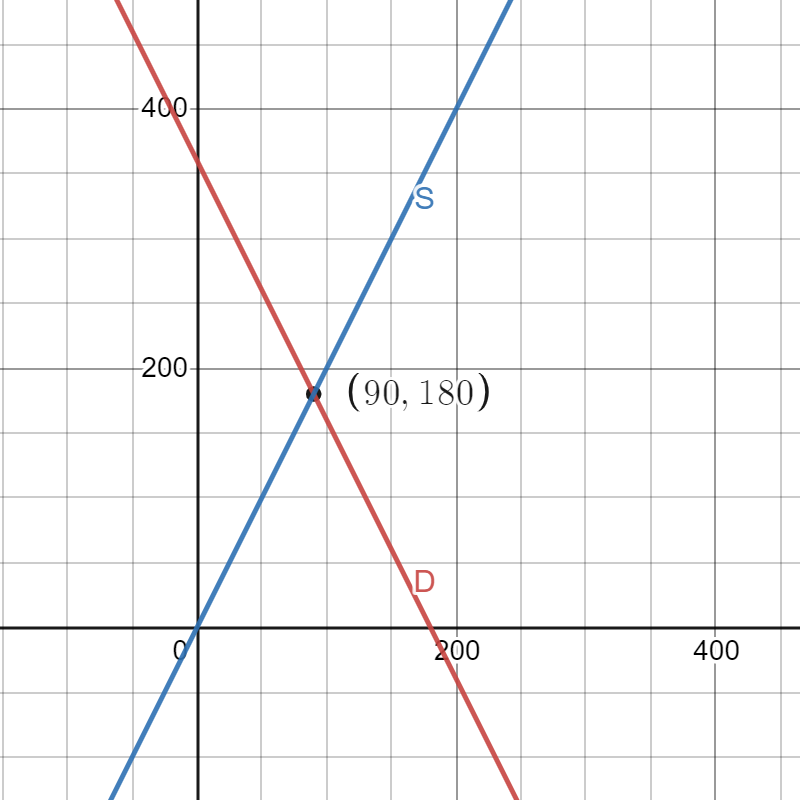
\includegraphics[width=5cm]{desmos mutual inelastic.png}
        \end{figure}
    \begin{itemize}[<+->]
        \item What do CS and PS look like in the picture above?
        \item Relatively large, compared to before
    \end{itemize}
\end{frame}


\begin{frame}{Example 2: Mutually Inelastic Supply (Computation)}
\begin{table}
\centering
\renewcommand{\arraystretch}{3}
\begin{tabu}{cc}
    \multirow{2}[2]{*}[2mm]{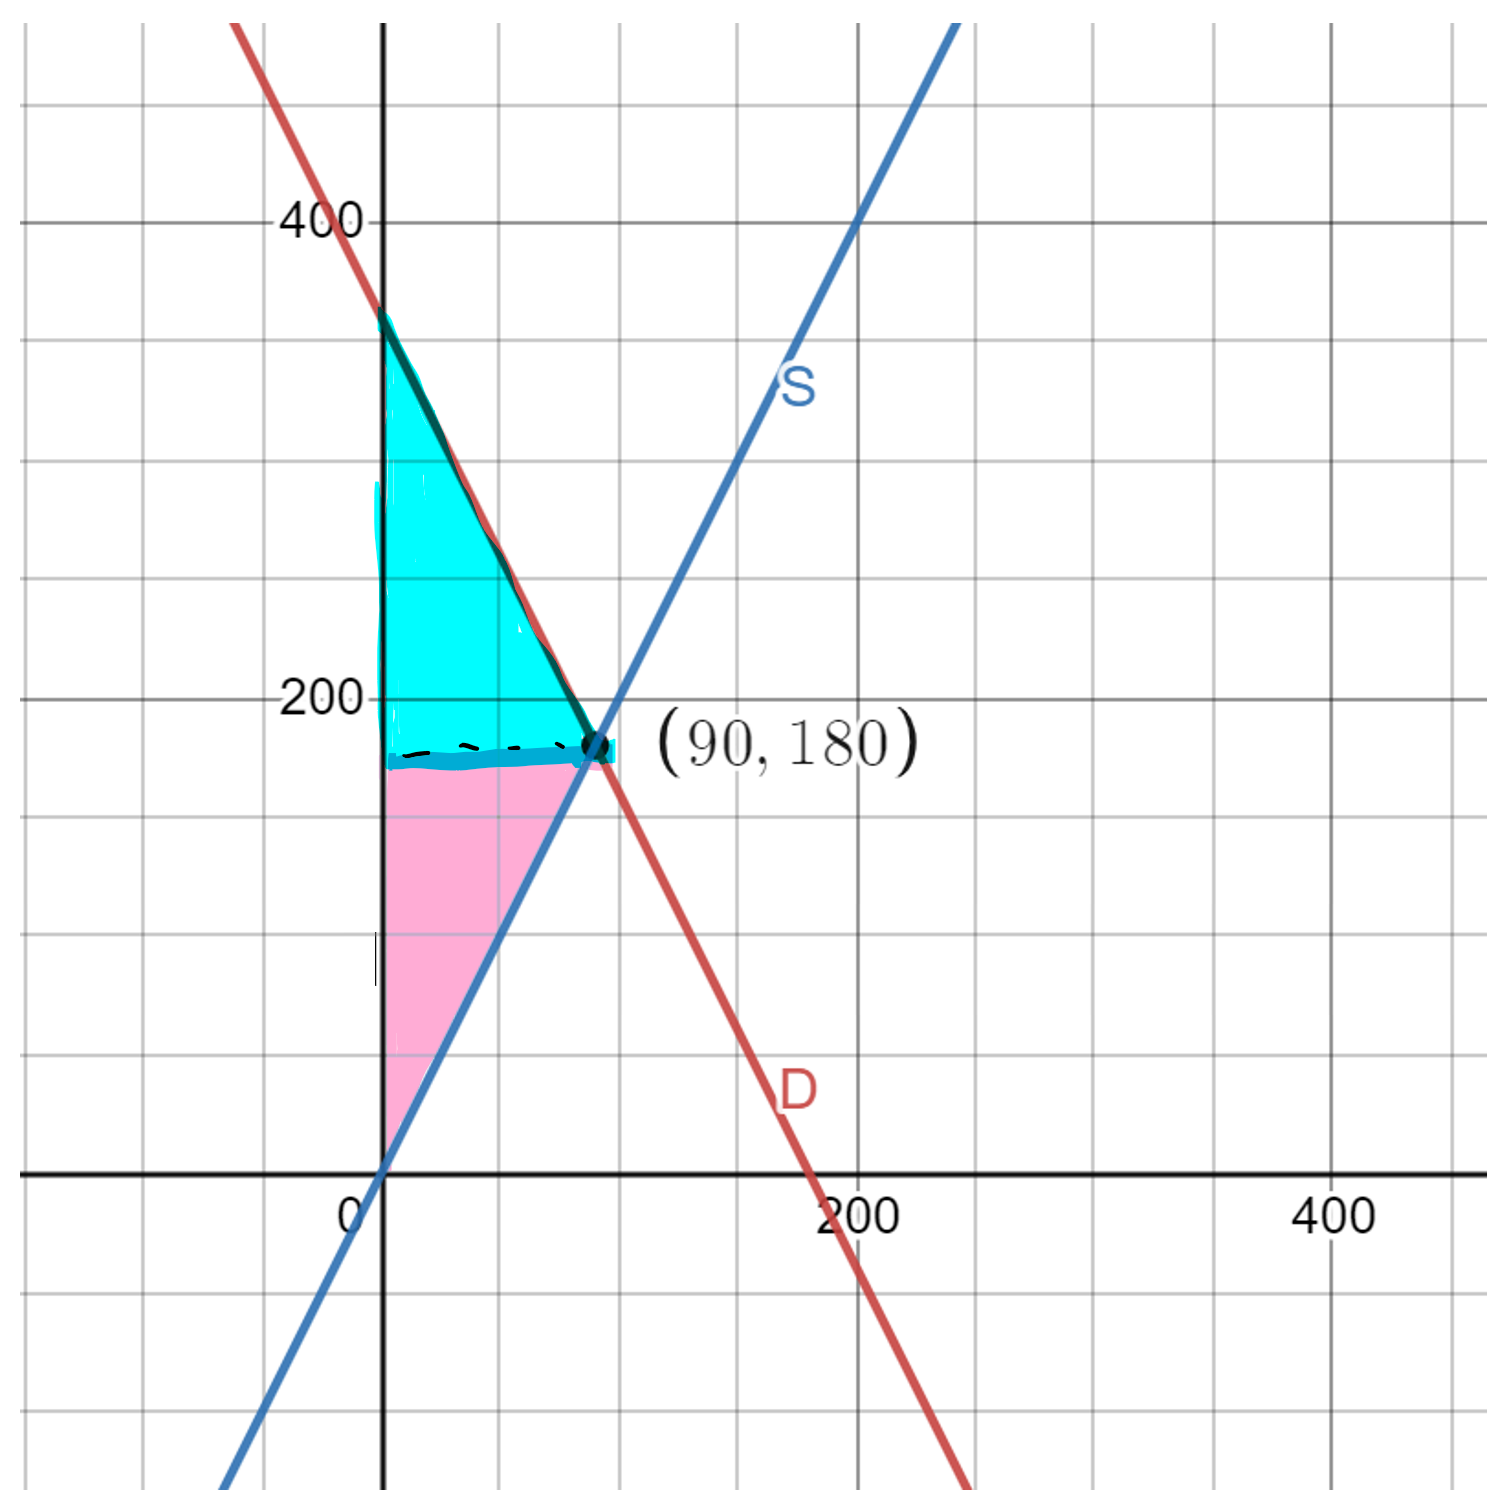
\includegraphics[width=4cm]{desmos mutual inelastic CS-PS.png}} & $[D]: \quad P=360-2Q$ \bigstrut \\
    & $[S]: \quad P=2Q$ \bigstrut\\
\end{tabu}
\end{table}
\vspace{8mm}
    \begin{itemize}[<+->]
        \item $CS=\frac{1}{2}(90)(360-180)=8100$
        \item $PS=\frac{1}{2}(90)(1800)=8100$
        \item What's happening: both consumers and producers are very willing to adapt to prices. Consequently, there is a large gap between their willingness to pay and the agreed upon price
    \end{itemize}
\end{frame}


\begin{frame}{Exercise: Elastic Demand and Inelastic Supply}
    \begin{itemize}[<+->]
        \item Now consider a market in with elastic demand but inelastic supply
        \begin{itemize}
            \item Consumers are relatively sensitive to changes in price, producers are not
            \item Suppliers really want to sell, consumers only barely want to buy
        \end{itemize}
        \item Let's combine the equations we have already worked with
        \begin{align*}
            [D]: \quad P&=189-\frac{1}{10}Q\\
            [S]: \quad P&=2Q
        \end{align*}
    \end{itemize}
\end{frame}

\begin{frame}{Exercise (Graph)}
        \begin{figure}
            \centering
            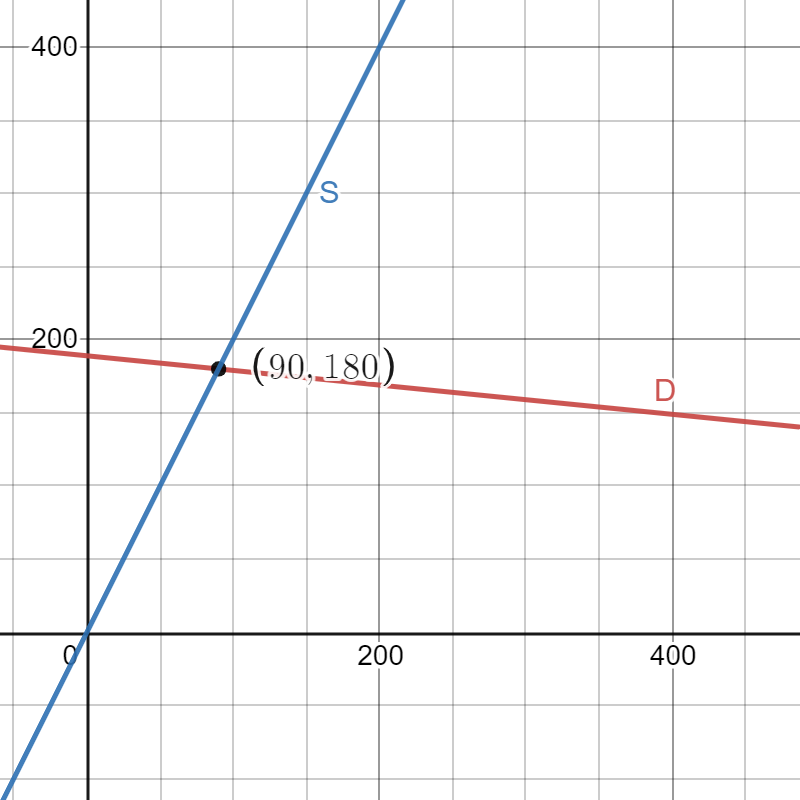
\includegraphics[width=5cm]{desmos elasticity ex3.png}
        \end{figure}
    \begin{itemize}[<+->]
        \item What do CS and PS look like in the picture above?
        \item CS is relatively large, PS is relatively small
    \end{itemize}
\end{frame}


\begin{frame}{Exercise (Computation)}
\begin{table}
\centering
\renewcommand{\arraystretch}{3}
\begin{tabu}{cc}
    \multirow{2}[2]{*}[2mm]{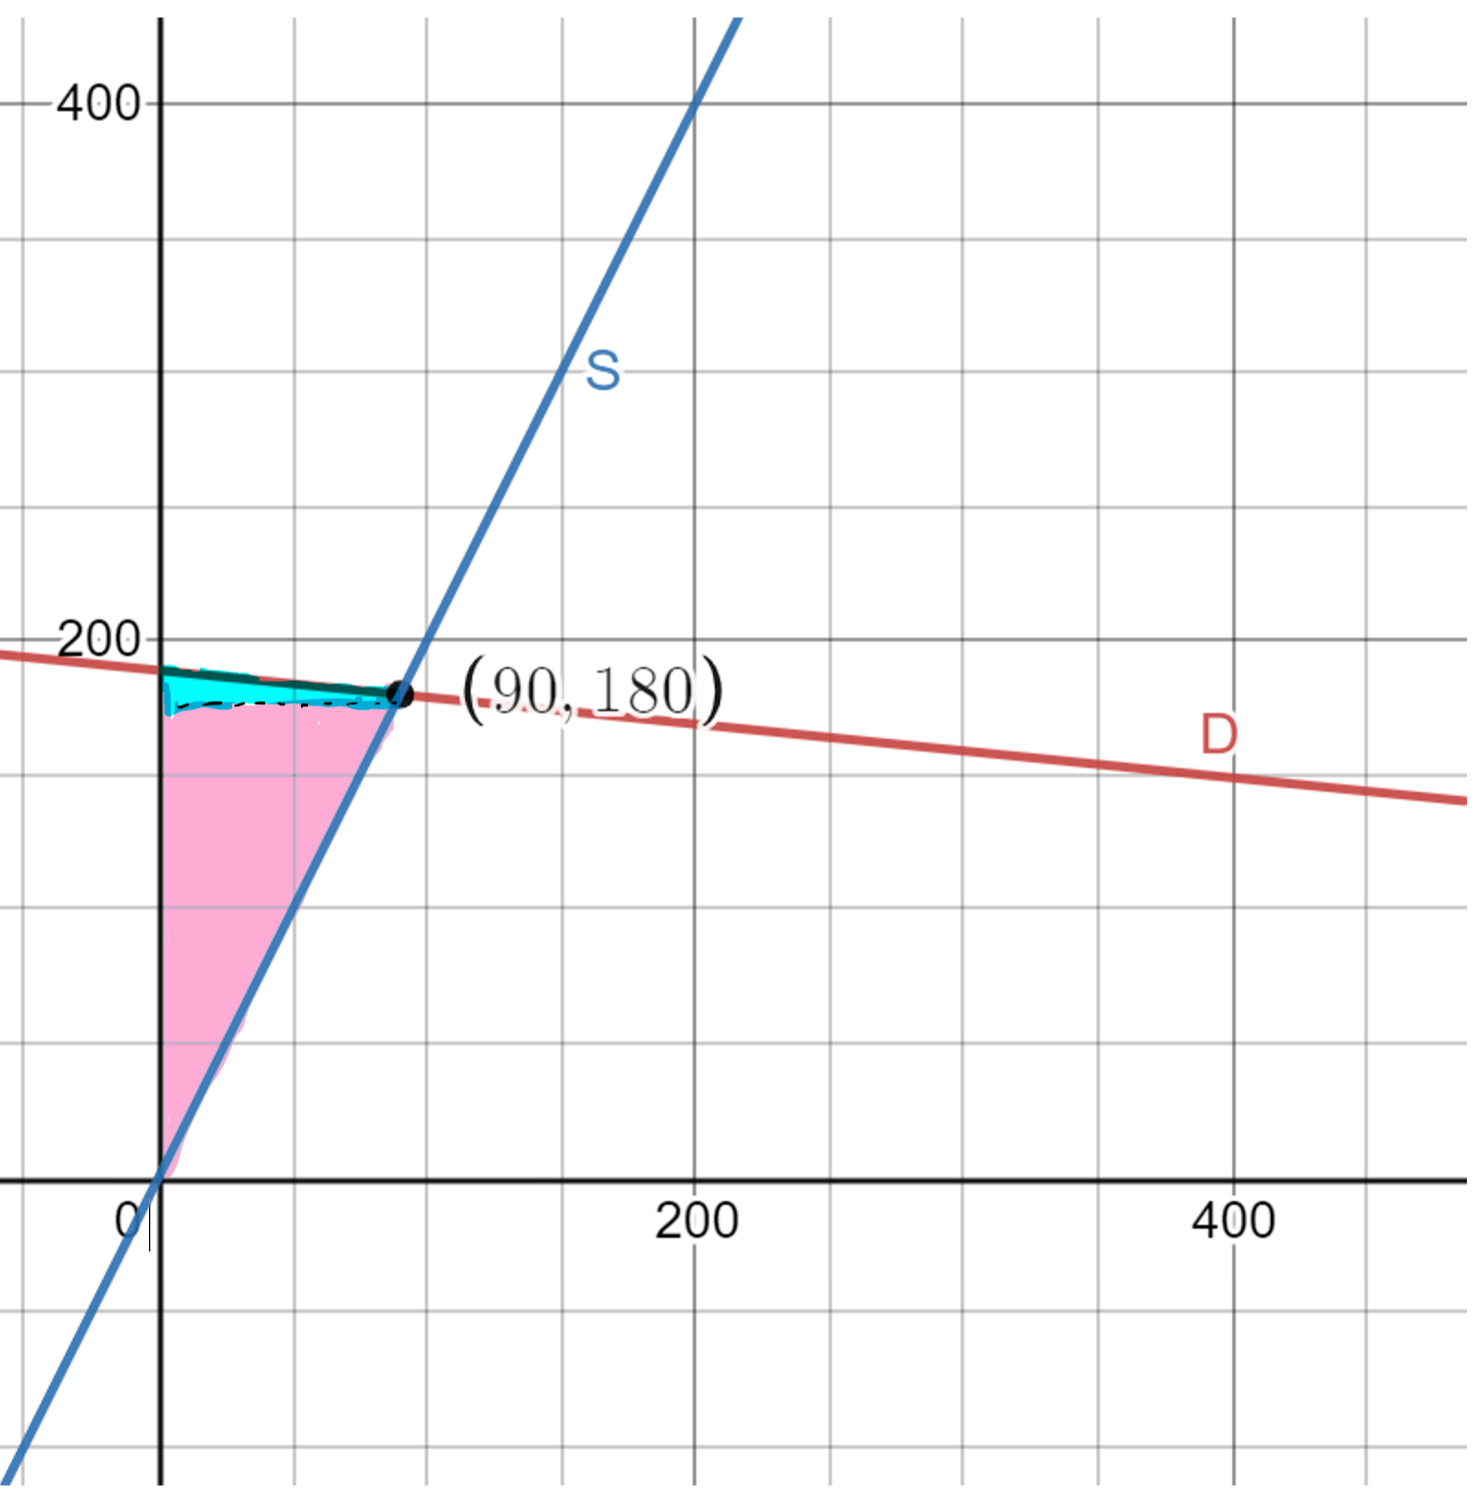
\includegraphics[width=4cm]{desmos elasticity ex3 CS-PS.png}} & $[D]: \quad P=189-\frac{1}{10}Q$ \bigstrut \\
    & $[S]: \quad P=2Q$ \bigstrut\\
\end{tabu}
\end{table}
\vspace{8mm}
    \begin{itemize}[<+->]
        \item $CS=405$
        \item $PS=8100$
        \item What's happening: producers really want to sell, while consumers are not that jazzed about buying
    \end{itemize}
\end{frame}

\begin{frame}{Takeaway}
    \begin{itemize}[<+->]
        \item Generally speaking, being insensitive to prices (price inelastic) will increase your (side of the market's) surplus value
        \item While being sensitive to prices (price elastic) will decrease your (side of the market's) surplus value
        \item If you want to get more familiar with these, play around with equations in desmos on your own
        \begin{itemize}
            \item Inelastic curves should be steep
            \item Elastic curves should be flat
            \item If you want to compare to equilibria, make them go through the same point
            \item For reference: \href{https://www.desmos.com/calculator/voucbuxux6}{Desmos from this section}
        \end{itemize}
        \item I want you to be prepared to see a graph you haven't seen before, make the surplus/elasticity computations, and make qualitative observations
    \end{itemize}
\end{frame}


\section*{Elasticity and Price Controls}

\begin{frame}{Ex 1: A Price Floor with Opposite Kinds of Elasticity}
    \begin{itemize}[<+->]
        \item  Consider a market with inelastic demand, but inelastic supply:
        \begin{align*}
            [D]: \quad P&=64-4Q\\
            [S]: \quad P&=31+\frac{1}{8}Q
        \end{align*}
        \item \underline{Challenge}: without looking at the graph given to you in the next slide, compute the equilibrium in this market, as well as CS and PS
    \end{itemize}
\end{frame}


\begin{frame}{Ex 1 (Graph)}
    \begin{figure}
        \centering
        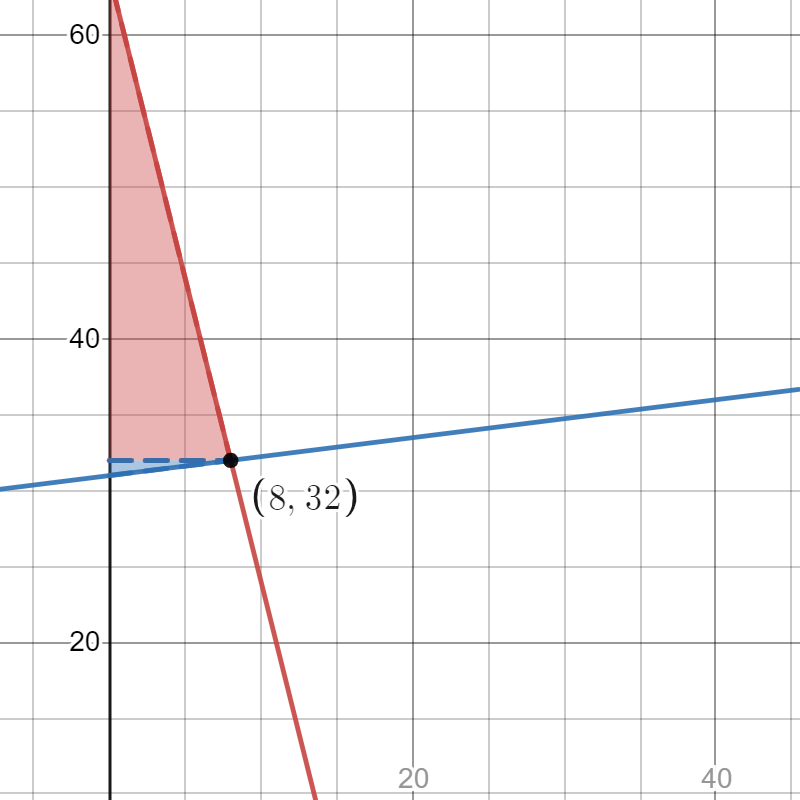
\includegraphics[width = 5cm]{elas cont ex1.png}
    \end{figure}
    \begin{itemize}[<+->]
        \item $CS=128$, $PS=4$
        \item What happens when we add a price floor?
    \end{itemize}
\end{frame}


\begin{frame}{Ex 1 (Floor)}
    \begin{table}[]
        \centering
        \begin{tabular}{c|c}
            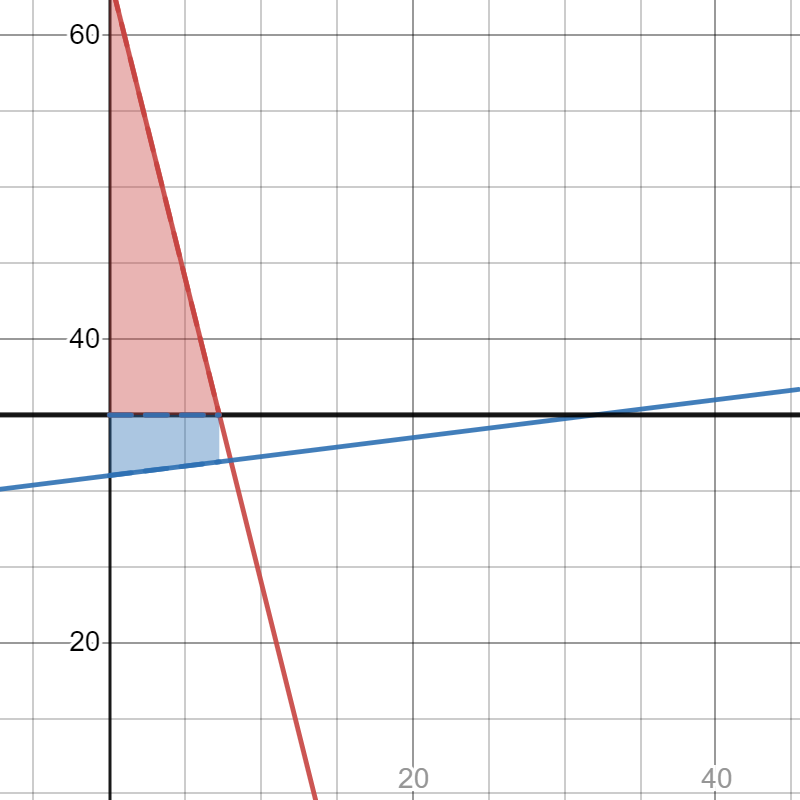
\includegraphics[width = 3.5cm]{desmos ex1 g1.png} & 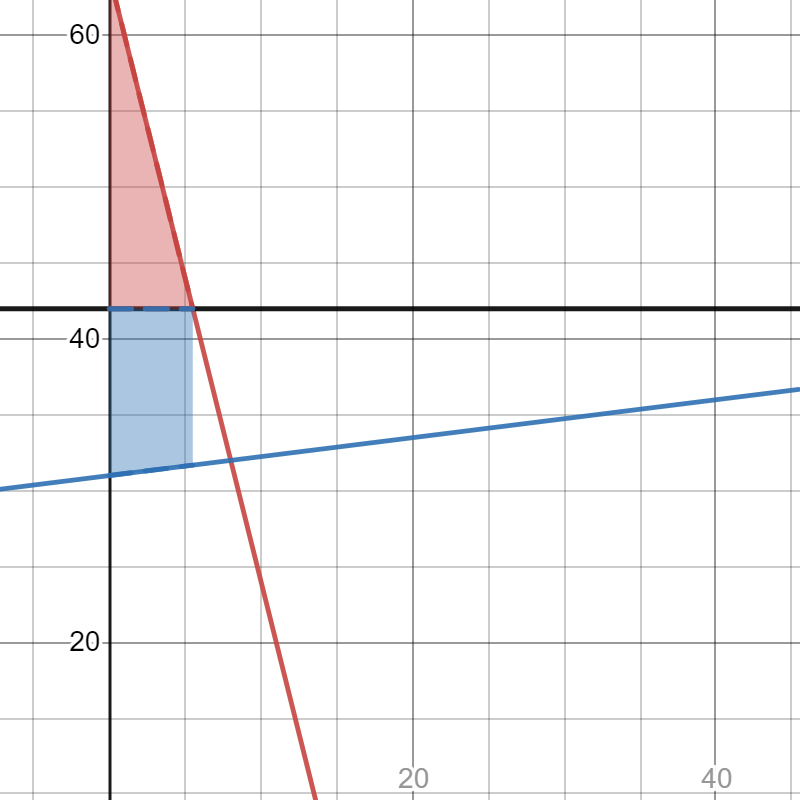
\includegraphics[width = 3.5cm]{desmos ex1 g2.png} 
        \end{tabular}
        \caption*{Price floors at $\$35$ and $\$42$, resp.}
    \end{table}
    \begin{itemize}[<+->]
        \item What does it look like is happening?
        \item CS is shrinking rapidly, much of it going to PS
        \item Since consumers have high valuations, they lose surplus quickly
        \item Conversely, since they are insensitive to prices, not many drop out, so much of the surplus goes to producers
    \end{itemize}
\end{frame}

\begin{frame}{Exercise 1: DWL Calculation}
    \begin{itemize}[<+->]
        \item When there is a price floor of $\$42$, find DWL:
        \begin{figure}
            \centering
            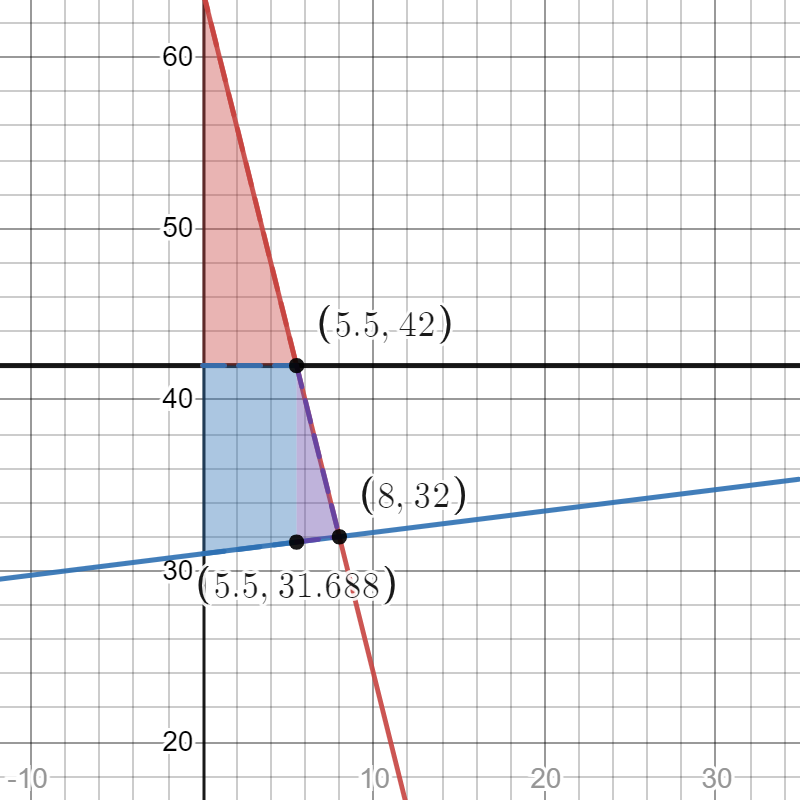
\includegraphics[width = 3.5cm]{desmos ex1 dwl.png}
        \end{figure}
        \item $DWL=\frac{1}{2}(8-5.5)(42-31.688)=12.89$
        \item If you want to play around with this (it's only set up for price floors, but you should able to visualize surpluses with ceilings): \href{https://www.desmos.com/calculator/8ivsmlqb1o}{Ex 1 Graph}
    \end{itemize}
\end{frame}


\begin{frame}{Ex 1 -- Food for Thought}
    \begin{figure}
        \centering
        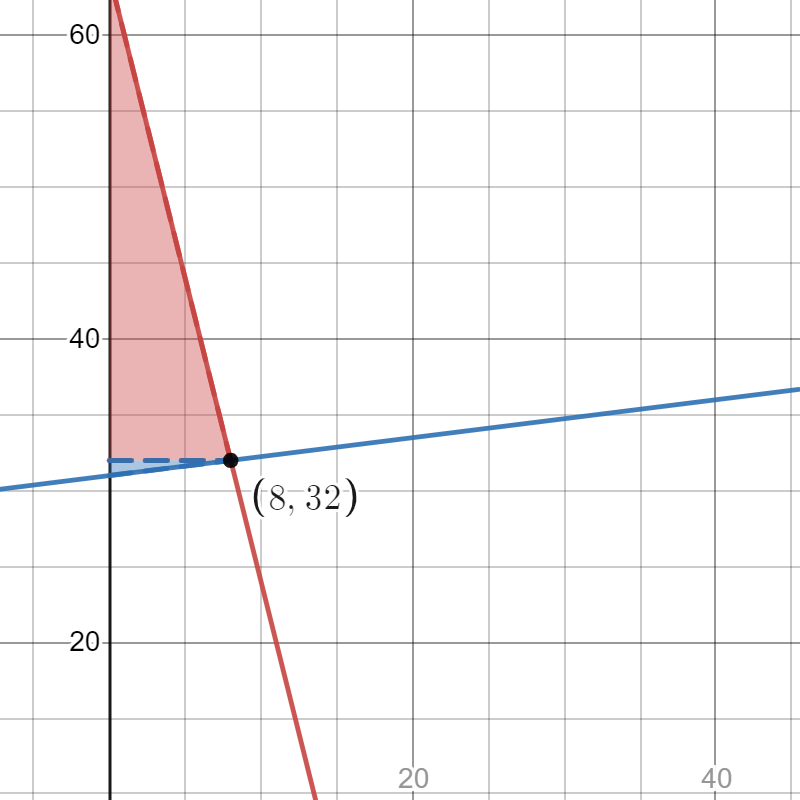
\includegraphics[width = 4cm]{elas cont ex1.png}
    \end{figure}
    \begin{itemize}[<+->]
        \item What would happen if we instead implemented a price ceiling in this case?
        \item PS will slowly shrink, some of it going to CS, some to deadweight loss
        \item Since producers have relatively low valuations, their PS doesn't have much more to fall. Meanwhile, since they are sensitive to price changes, they will fall out of the market quickly, limiting the growth of consumer surplus
    \end{itemize}
\end{frame}

\begin{frame}{Example 2: A Price Ceiling with Varying Elasticities}
    \begin{itemize}[<+->]
        \item  Consider a market with elastic demand, but inelastic supply:
        \begin{align*}
            [D]: \quad P&=34-\frac{1}{4}Q\\
            [S]: \quad P&=8+3Q
        \end{align*}
        \item \underline{Challenge}: without looking at the graph given to you in the next slide, compute the equilibrium in this market, as well as CS and PS
    \end{itemize}
\end{frame}

\begin{frame}{Ex 2 (Graph)}
    \begin{figure}
        \centering
        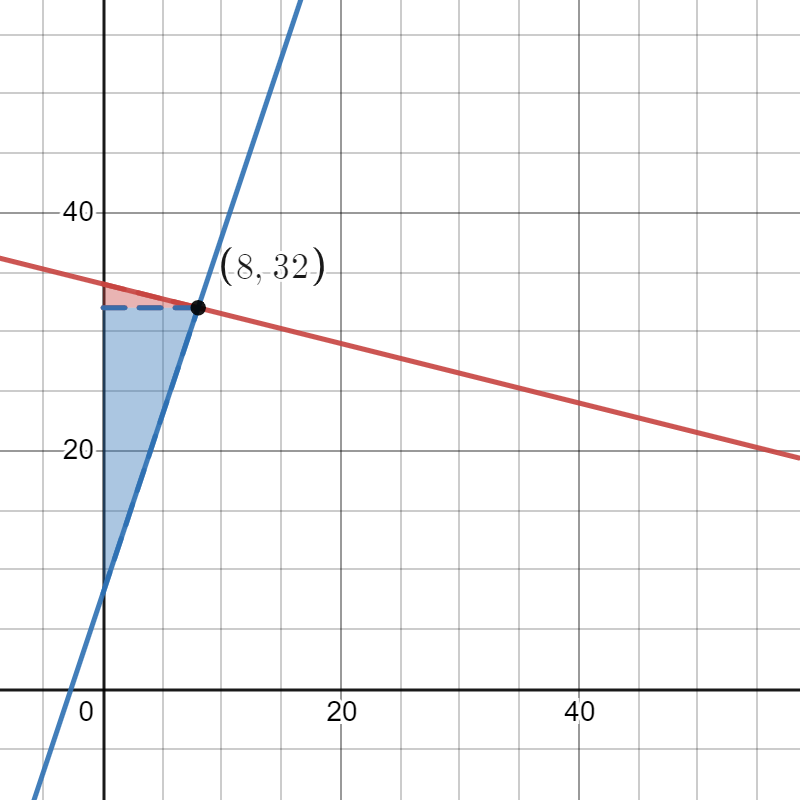
\includegraphics[width = 5cm]{elas cont ex2.png}
    \end{figure}
    \begin{itemize}[<+->]
        \item $CS=8$, $PS=96$
        \item What happens when we add a price ceiling?
    \end{itemize}
\end{frame}

\begin{frame}{Ex 2 (Floor)}
    \begin{table}[]
        \centering
        \begin{tabular}{c|c}
            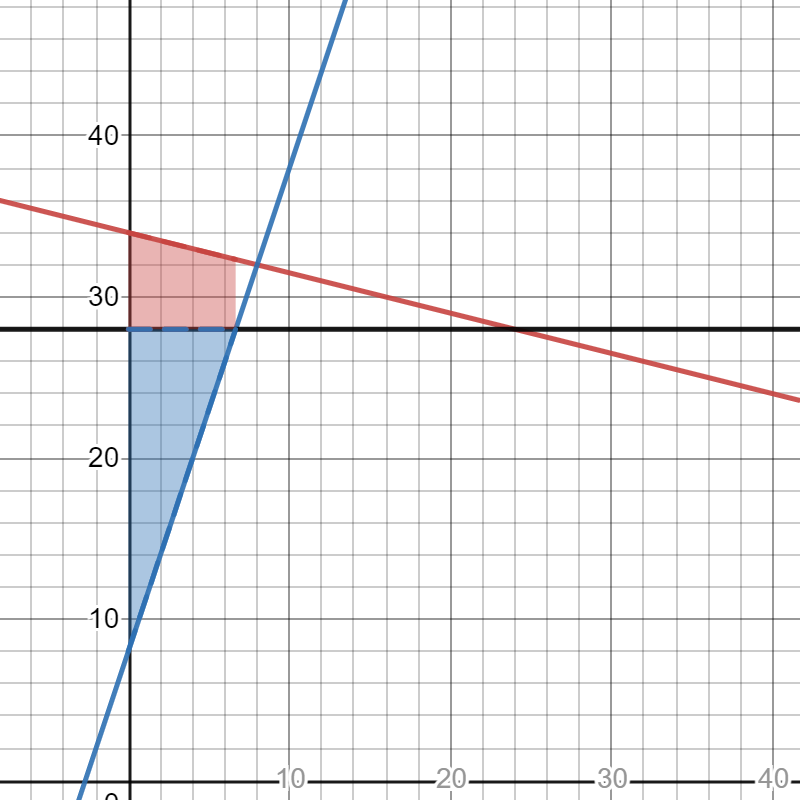
\includegraphics[width = 3.5cm]{desmos ex2 g1.png} & 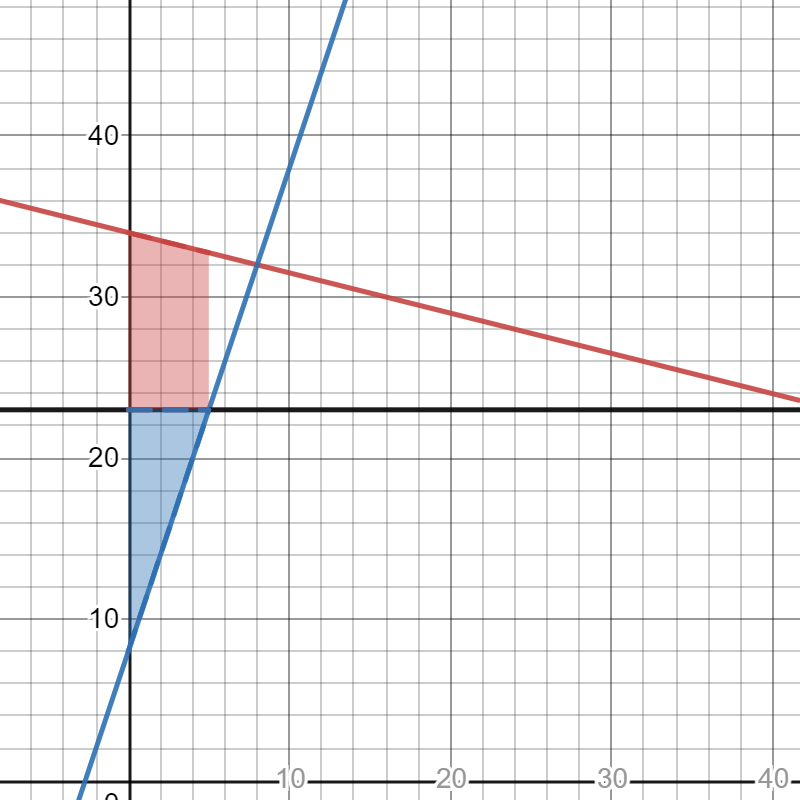
\includegraphics[width = 3.5cm]{desmos ex2 g2.png} 
        \end{tabular}
        \caption*{Price ceilings at $\$23$ and $\$28$, resp.}
    \end{table}
    \begin{itemize}[<+->]
        \item What does it look like is happening?
        \item PS is shrinking rapidly, much it going to CS
        \item Since producers have high valuations, they lose surplus quickly
        \item Conversely, since they are insensitive to prices, not many drop out, so much of the surplus goes to consumers
    \end{itemize}
\end{frame}

\begin{frame}{Exercise 1: DWL Calculation}
    \begin{itemize}[<+->]
        \item When there is a price ceiling of $\$28$, find DWL:
        \begin{figure}
            \centering
            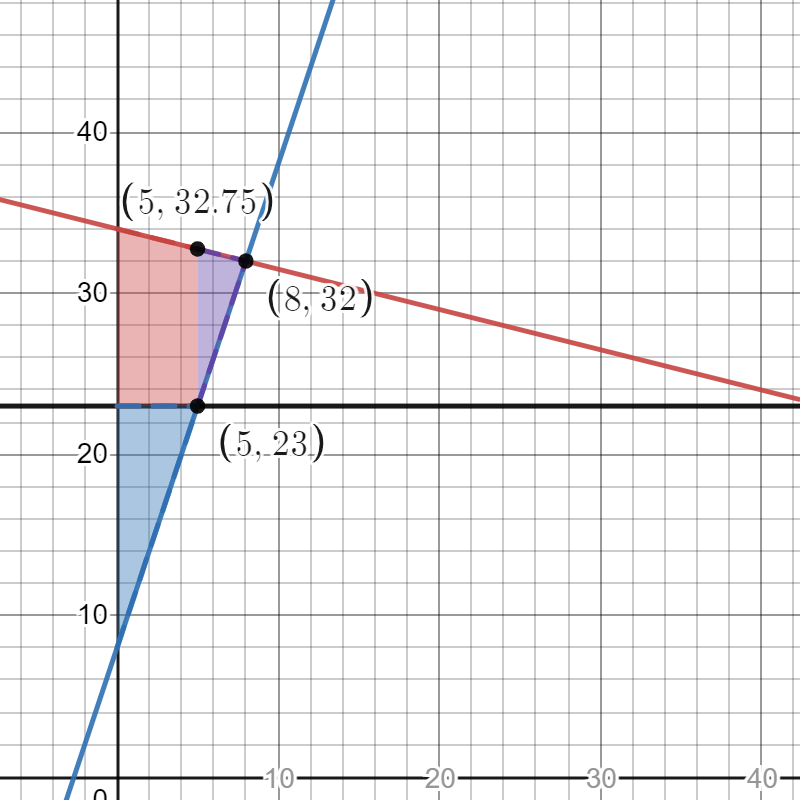
\includegraphics[width = 3.5cm]{desmos ex2 dwl.png}
        \end{figure}
        \item $DWL=\frac{1}{2}(8-5)(32.75-23)=14.65$
        \item If you want to play around with this (it's only set up for price floors, but you should able to visualize surpluses with ceilings): \href{https://www.desmos.com/calculator/c8t0as5qik}{Ex 2 Graph}
    \end{itemize}
\end{frame}


\begin{frame}{Ex 2 -- Food for Thought}
    \begin{figure}
        \centering
        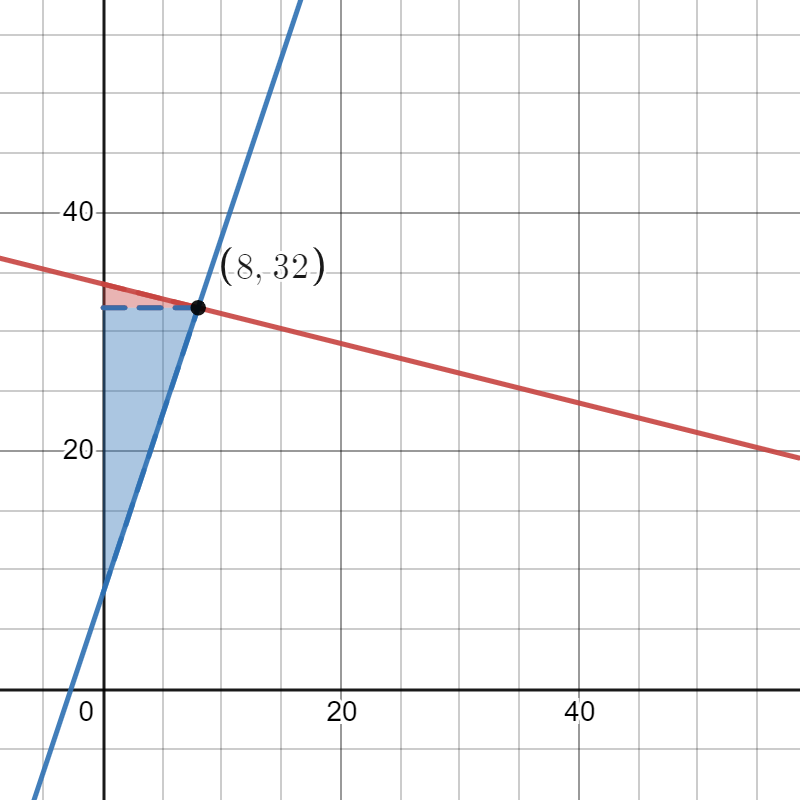
\includegraphics[width = 4cm]{elas cont ex2.png}
    \end{figure}
    \begin{itemize}[<+->]
        \item What would happen if we instead implemented a price floor in this case?
        \item CS will slowly shrink, some of it going to PS, some of it going to DWL
    \end{itemize}
\end{frame}


\begin{frame}{Takeaway}
    \begin{itemize}[<+->]
        \item Elasticities affect both price controls and welfare
        \item By looking at a graph, and/or given numbers, I would like you to be able to perform welfare calculations, and make qualitative observations
        \item Keep sensitivity to prices in mind, as well as the fact that inelastic demand usually means relatively high valuations/enjoyment for products (similar for supply)
        \item Make sure you know how to calculate DWL
    \end{itemize}
\end{frame}





\section*{Midterm Discussion}
\begin{frame}{Logistics}
    \begin{itemize}[<+->]
        \item Midterm is a week from today -- Wednesday, November 3rd 
        \begin{itemize}
            \item Bring non-graphing, non-algebra calculator
            \item Bring \#2 Pencil (yes it has to be \#2)
            \item BRING PICTURE ID, there will be a seating chart
        \end{itemize}
        \item Read the announcement about class-designed note card
        \begin{itemize}
            \item I need the finished community note card to be done by this coming Monday night (Tuesday is fine, but I need to make sure everyone has time to approve finishing touches)
            \item One sheet, not front/back
        \end{itemize}
    \end{itemize}
\end{frame}

\begin{frame}{Logistics (cont.)}
    \begin{itemize}[<+->]
        \item Rough format:\footnote{No guarantees}
        \begin{itemize}
            \item 30-40 MC questions (probably closer to 40)
            \item 4-7 free response questions (probably closer to 4)
        \end{itemize}    
        \item At 40 MC questions, 4 free response, managing your 80 minutes will mean $\approx$ 1.5 minutes (\underline{average})/MC question, plus $\approx$ 5 minutes per free response question
        \item I will announce the specific \# MC/FR questions closer to the test, and what the breakdown comes out to
    \end{itemize}
\end{frame}

\begin{frame}{Basic Overview of Topics}
    \begin{itemize}[<+->]
        \item The following list is a brief overview, and is by no means extensive
        \item PPF and OC
            \begin{itemize}
                \item Draw a PPF given production table, understand it's regions
                \item Shifting a PPF
                \item Compute OC from production table
                \item Combine two PPFs from trade 
            \end{itemize}
        \item Demand Curve (Supply curve, resp.)
            \begin{itemize}
                \item How to draw one from data
                \item Individual curves $\to$ market curve
                \item What causes movement along, what shifts
                \item Law of demand (supply)
                \item Graphing with equations
            \end{itemize}
        \item Equilibrium
            \begin{itemize}
                \item Identifying, intuition behind markets
                \item Shifting both supply and demand, and seeing the impact on equilibrium $P$ and $Q$
                \item Graphing
            \end{itemize}
    \end{itemize}
\end{frame}

\begin{frame}{Basic Overview of Topics (cont.)}
    \begin{itemize}[<+->]
        \item Elasticity 
            \begin{itemize}
                \item PED, Income elasticity of demand, CPED, Price elasticity of supply
                \item How to compute given data/points on graph
                \item How to interpret
                \item Steep curve usually implies relatively inelastic
                \item Can vary along linear demand curve
                \item Ceteris Paribus
            \end{itemize}
        \item CS/PS
            \begin{itemize}
                \item Identification
                \item Interpretation
                \item How to calculate it
                \item How they are influenced by relative elasticity
                \item TWTP and MWTP tables, diminishing marginal returns
            \end{itemize}
        \item Price Ceilings/Floors
            \begin{itemize}
                \item Identification, including effective/ineffective
                \item Effect on market, including new price, $Q_{D}$, $Q_{s}$, and quantity traded
                \item Shortages and surpluses, including how to calculate them
                \item Effect on market
            \end{itemize}
    \end{itemize}
\end{frame}

\begin{frame}{Resources}
    \begin{itemize}[<+->]
        \item Cengage Chapter Sections titled "review for the test"
        \item Office hours -- either in person or by appointment
        \item Discussion section this Friday will be reserved for review
        \item Review the slides and homework, read the book
        \item Questions?
    \end{itemize}
\end{frame}


\end{document}